\chapter{Visión Artificial}
\cleanchapterquote{Let's go invent tomorrow instead of worrying about what happened yesterday.}{Steve Jobs}{(American business magnate, industrial designer, investor, and media proprietor.)}

\section{Cámara}
Como se abordó al inicio de este proyecto, la cámara es la parte fundamental en
la captura de datos, suple la función de un ojo y depende de diversos
parámetros el que tengamos una captura de calidad. Para este trabajo profesional
la cámara que se utilizó fue la del fabricante HardKernel y que lleva de nombre
Ocam.
\begin{center}
	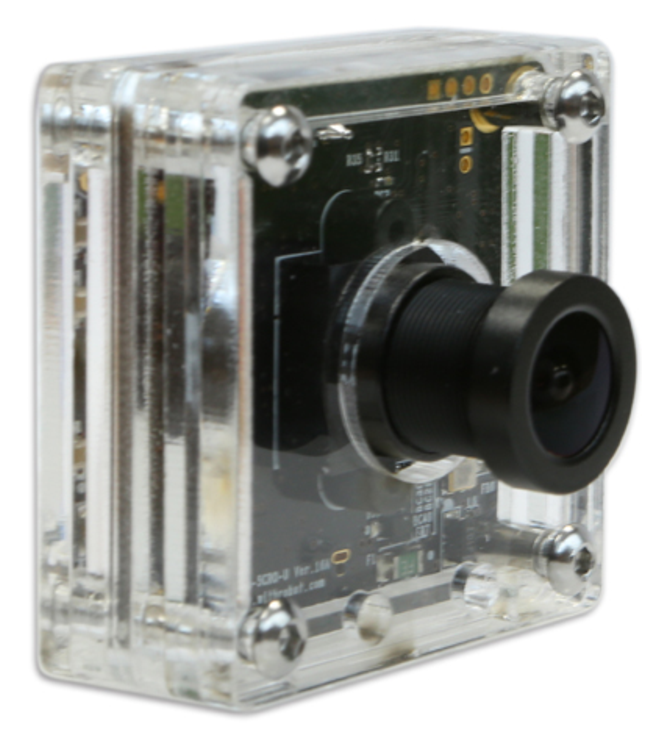
\includegraphics[width=0.3\textwidth]{Contenido/Cuerpo/Capitulo4/Fig0_1.eps}
	\captionof{figure}{Cámara 'Ocam' obtenida de \cite{WEB:Ocam}}\label{Fig1}
\end{center}
Que tiene las siguientes especificaciones.
\begin{itemize}
	\item \textbf{Sensor:} CMOS image sensor.
	\item \textbf{Lente: } Lente estandar M12 distancia focal de 3.6mm.
	\item \textbf{Field of view: } 65 grados.
	\item \textbf{Tamaño del sensor: }0.25inch (3673.6 $\mu$m x 2738.4 $\mu$m)
	\item \textbf{Tamaño del pixel: } 1.4 $\mu$m x 1.4 $\mu$m.
	\item \textbf{Interfaz: }USB 3.0 Super-Speed.
	\item \textbf{Frame rate: }\\
	      1920 x 1080 a 30fps, 1280 x 720 a45fps, 640 x 480 a30fps
\end{itemize}
El acceso directo a la memoria a través de USB 3.0 permite que los datos se
escriban en la memoria principal sin pasar por la CPU. Reduce significativamente
la carga de trabajo de la CPU.

% ---------------------------------------------------------------------------------------------------------
% *********************************************************************************************************
% *********************************************************************************************************
% ---------------------------------------------------------------------------------------------------------

\section{Algoritmo general}
El proceso de la obtención del centroide de la figura requiere seguir una serie de pasos relacionados con el
procesamiento de imágenes, podemos entonces definir esos pasos como un algoritmo, descrito en la siguiente lista.

\begin{algorithm}
	\caption{Obtener centroide de figura}
	\begin{algorithmic}[1]
		\State{Calibrar cámara}
		\State{Capturar frames a 60fps}
		\State{Publicar frames en ROS}
		\State{Corrección de brillo y saturación}
		\State{Convertir RGB a HSV}
		\State{Acotar el modelo HSV al color de elección}
		\State{Agregar filtro morfológico}
		\State{Obtener centroide de la figura obtenida en 7 con función moments de openCV}
		\State{Publicar coordenadas del centroide}
	\end{algorithmic}
\end{algorithm}


% ---------------------------------------------------------------------------------------------------------
% *********************************************************************************************************
% *********************************************************************************************************
% ---------------------------------------------------------------------------------------------------------


\section{Comunicación con ROS}
En la sección de vision artificial se lanzan dos nodos, uno encargado de capturar y
publicar frames a 60hz y el otro que se suscribe a dicho nodo y realiza un procesamiento
con la información obtenida para posterior publicar coordenadas.
\begin{center}
	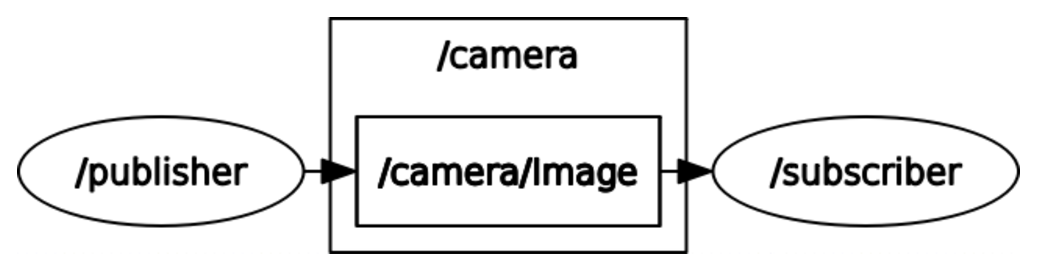
\includegraphics[width=0.6\textwidth]{Contenido/Cuerpo/Capitulo4/Fig0.eps}
	\captionof{figure}{Nodos y topic}\label{Fig1}
\end{center}
En la figura 4.1 se puede observar dos nodos conectados por un topic llamado /Image
encargado de comunicar la imagen de un nodo a otro.
\subsection{Publisher}
Como vimos anteriormente opencv es una librería open-source que se encarga del procesamiento
de imágenes, también abordamos un poco acerca de como ROS comunica nodos y los
tipos de datos que pueden ser publicados. Al hablar de que se va a publicar una imagen
estamos refiriéndonos a una matriz que en este caso sera de 640 x 480.\\
ROS pasa las imágenes en su propio formato sensor\_msgs/Image, pero
en este caso usaremos ROS junto con las librerías de OpenCV. CvBridge es una
biblioteca ROS que proporciona una interfaz entre ROS y OpenCV.
\begin{center}
	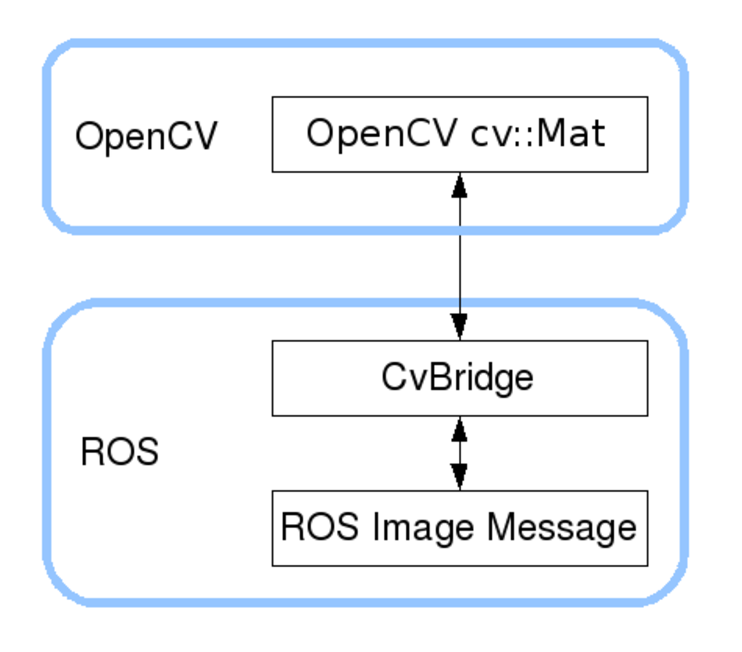
\includegraphics[width=0.4\textwidth]{Contenido/Cuerpo/Capitulo4/Fig1.eps}
	\captionof{figure}{Comunicación entre opencv y ROS}\label{Fig1}
\end{center}
Al convertir un mensaje sensor\_msgs/Image en una imagen Cv, CvBridge
reconoce dos casos de uso distintos:
\begin{itemize}
	\item Queremos modificar los datos en el lugar.\\
	      \textbf{Tenemos que hacer una copia de los datos del mensaje ROS.}
	\item No modificaremos los datos.\\
	      \textbf{Podemos compartir con seguridad los datos que posee el mensaje ROS en lugar de copiarlos.}
\end{itemize}
La entrada es el puntero del mensaje de imagen, así como un argumento de
codificación opcional. La codificación se refiere al destino CvImage.\\
Para codificaciones de imágenes populares, CvBridge opcionalmente realizará
conversiones de color o profundidad de píxeles según sea necesario. Para este proyecto
se utiliza bgr8: CV\_8UC3, es decir, que el orden del color es Azul, Verde y Rojo.\\
Con el fin de entender este nodo se hizo el siguiente diagrama de flujo:
\begin{center}
	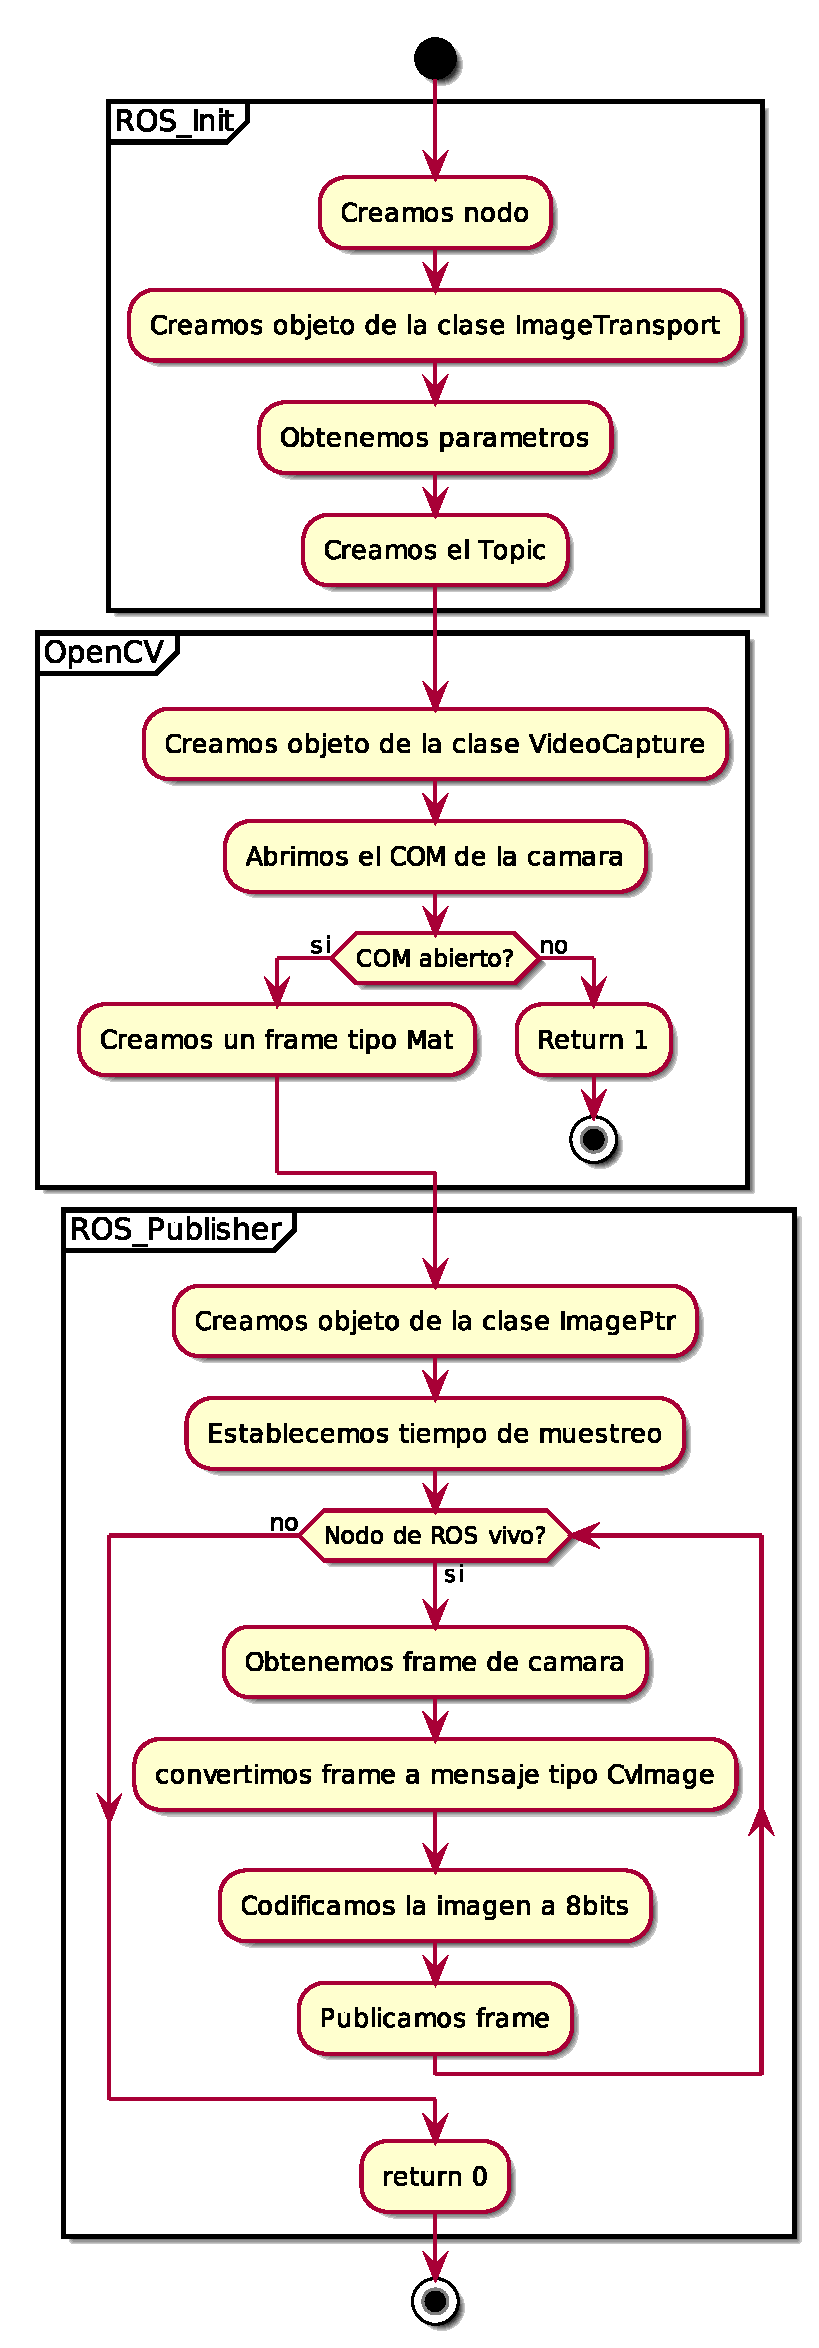
\includegraphics[width=0.6\textwidth]{Contenido/Cuerpo/Capitulo4/publisher.eps}
	\captionof{figure}{Diagrama de flujo del programa publisher}\label{Fig5}
\end{center}
El código se encuentra en la parte del Apéndice A, 'código 1'

\subsection{Subscriber}
Este nodo tiene dos funciones principales, Suscribirse al nodo publisher y publicar
un array de tamaño 2, tipo entero que guardara las coordenadas en X y Y del centroide
del objetivo.\\
El proceso que se ejecuta sé vera más a detalle en las siguientes secciones de este
capítulo.\\
Dichos procesos están incluidos en una clase llamada 'objectTracking' que se ilustra
en el siguiente diagrama.
\begin{center}
	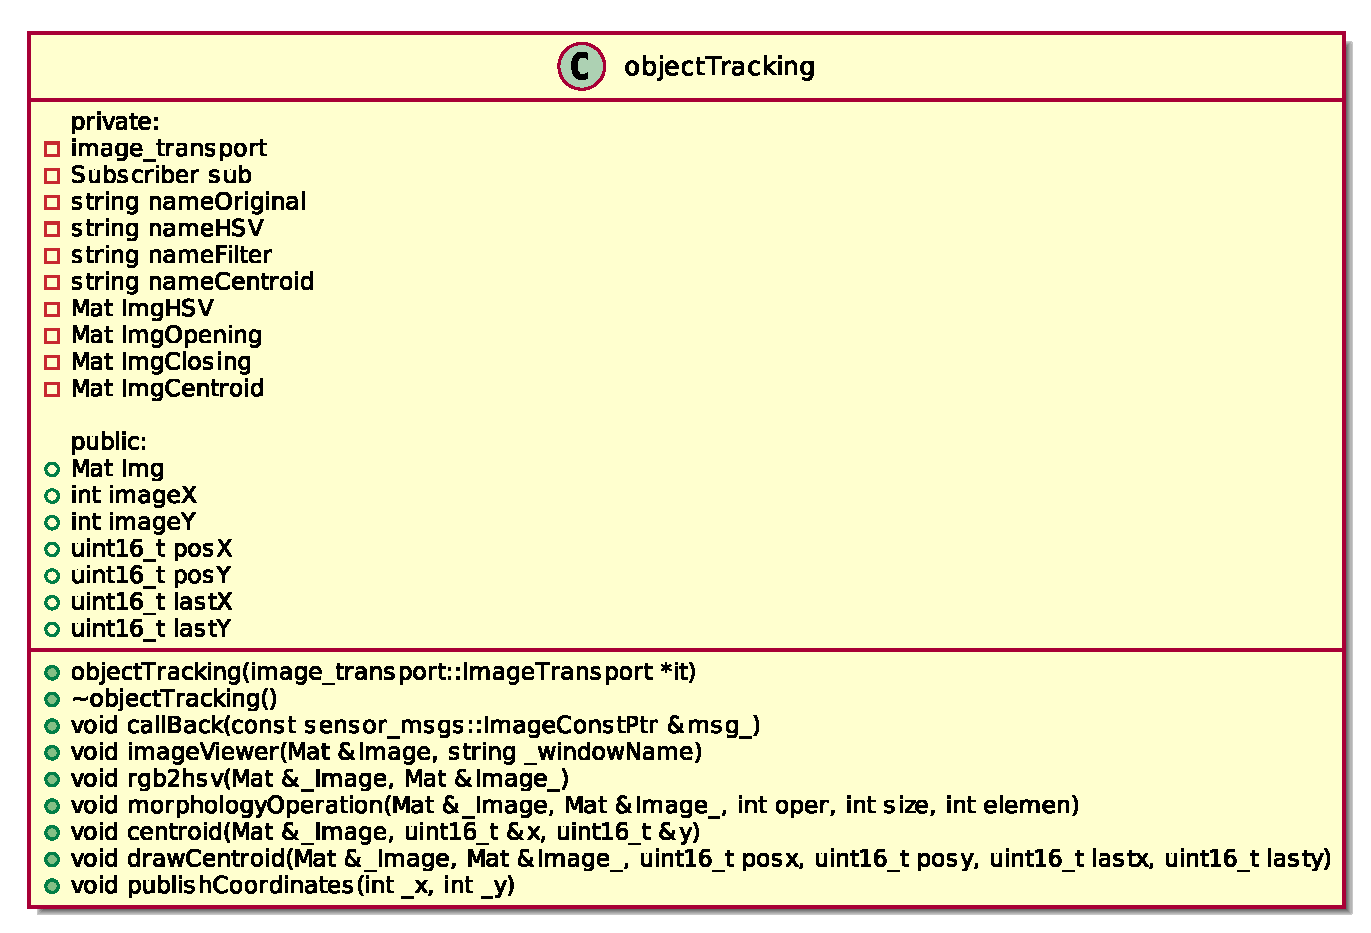
\includegraphics[width=0.45\textwidth]{Contenido/Cuerpo/Capitulo4/object_tracking.eps}
	\captionof{figure}{Diagrama de clases del subscriber}\label{Fig5}
\end{center}


% ---------------------------------------------------------------------------------------------------------
% *********************************************************************************************************
% *********************************************************************************************************
% ---------------------------------------------------------------------------------------------------------

\section{Calibración de camara}
Siguiendo la calibración basada en el algoritmo de Zhangs, previamente descrito en el capítulo 2,
comenzamos por posicionar la cámara en una mesa fija y colocando un tablero de ajedrez de dimensión
2.65 x 2.6cm cada cuadrito.\\ Lanzando los nodos de ROS y graficando en RQT
\begin{center}
	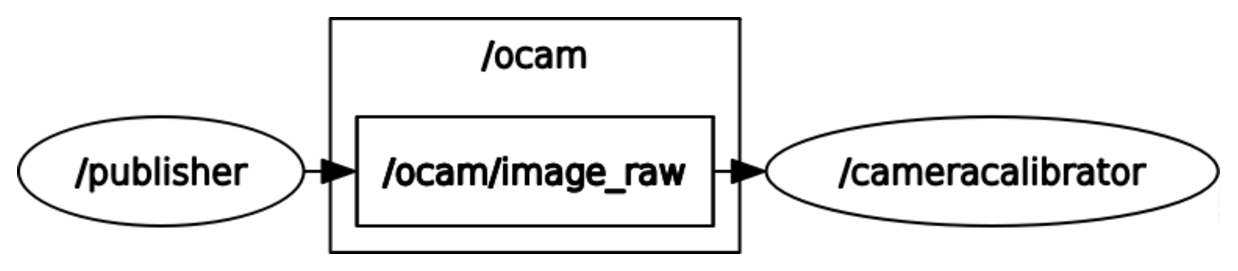
\includegraphics[width=0.5\textwidth]{Contenido/Cuerpo/Capitulo4/Fig11.eps}
	\captionof{figure}{Comunicación ROS con calibrador}\label{Fig1}
\end{center}

Para obtener una buena calibración, se movió el tablero de ajedrez en el marco de la cámara de
la siguiente manera:
\begin{itemize}
	\item Tablero de ajedrez a la izquierda, derecha, arriba y abajo del campo de visión de la cámara
	      \begin{itemize}
		      \item Barra X - izquierda / derecha en el campo de visión
		      \item Barra Y - arriba / abajo en el campo de visión
		      \item Barra de tamaño: hacia / lejos e inclinación de la cámara
	      \end{itemize}
	\item Tablero de ajedrez que llena todo el campo de visión
	\item Tablero de ajedrez inclinado hacia la izquierda, derecha, arriba y abajo (sesgado)
\end{itemize}
Tal como se ilustra en la siguiente figura
\begin{center}
	
\includegraphics[width=0.5\textwidth]{Contenido/Cuerpo/Capitulo4/Fig12.eps}
	\captionof{figure}{Proceso de calibración utilizando un tablero de ajedrez}\label{Fig1}
\end{center}
Despues del proceso de calibración los resultados son los siguientes:
Matriz de distorsión D[]
\begin{equation}
	D=
	\begin{bmatrix}
		-0.439076 & 0.215870 & 0.001905 & 0.005790 & 0.000000
	\end{bmatrix}
\end{equation}
Matriz de parámetros intrínsecos de la cámara
\begin{equation}
	K=
	\begin{bmatrix}
		656.41089 & 0         & 320.06053 \\
		0.        & 654.93593 & 222.93267 \\
		0.        & 0         & 1
	\end{bmatrix}
\end{equation}

Matriz de proyección de cámara P
\begin{equation}
	P=
	\begin{bmatrix}
		581.95032 & 0.        & 324.43609 & 0. \\
		0.        & 613.90649 & 221.23437 & 0. \\
		0.        & 0.        & 1.        & 0.
	\end{bmatrix}
\end{equation}
Una vez cambiando los parametros anteriores al pubicador da como resultado la sguiente imagen
\begin{center}
	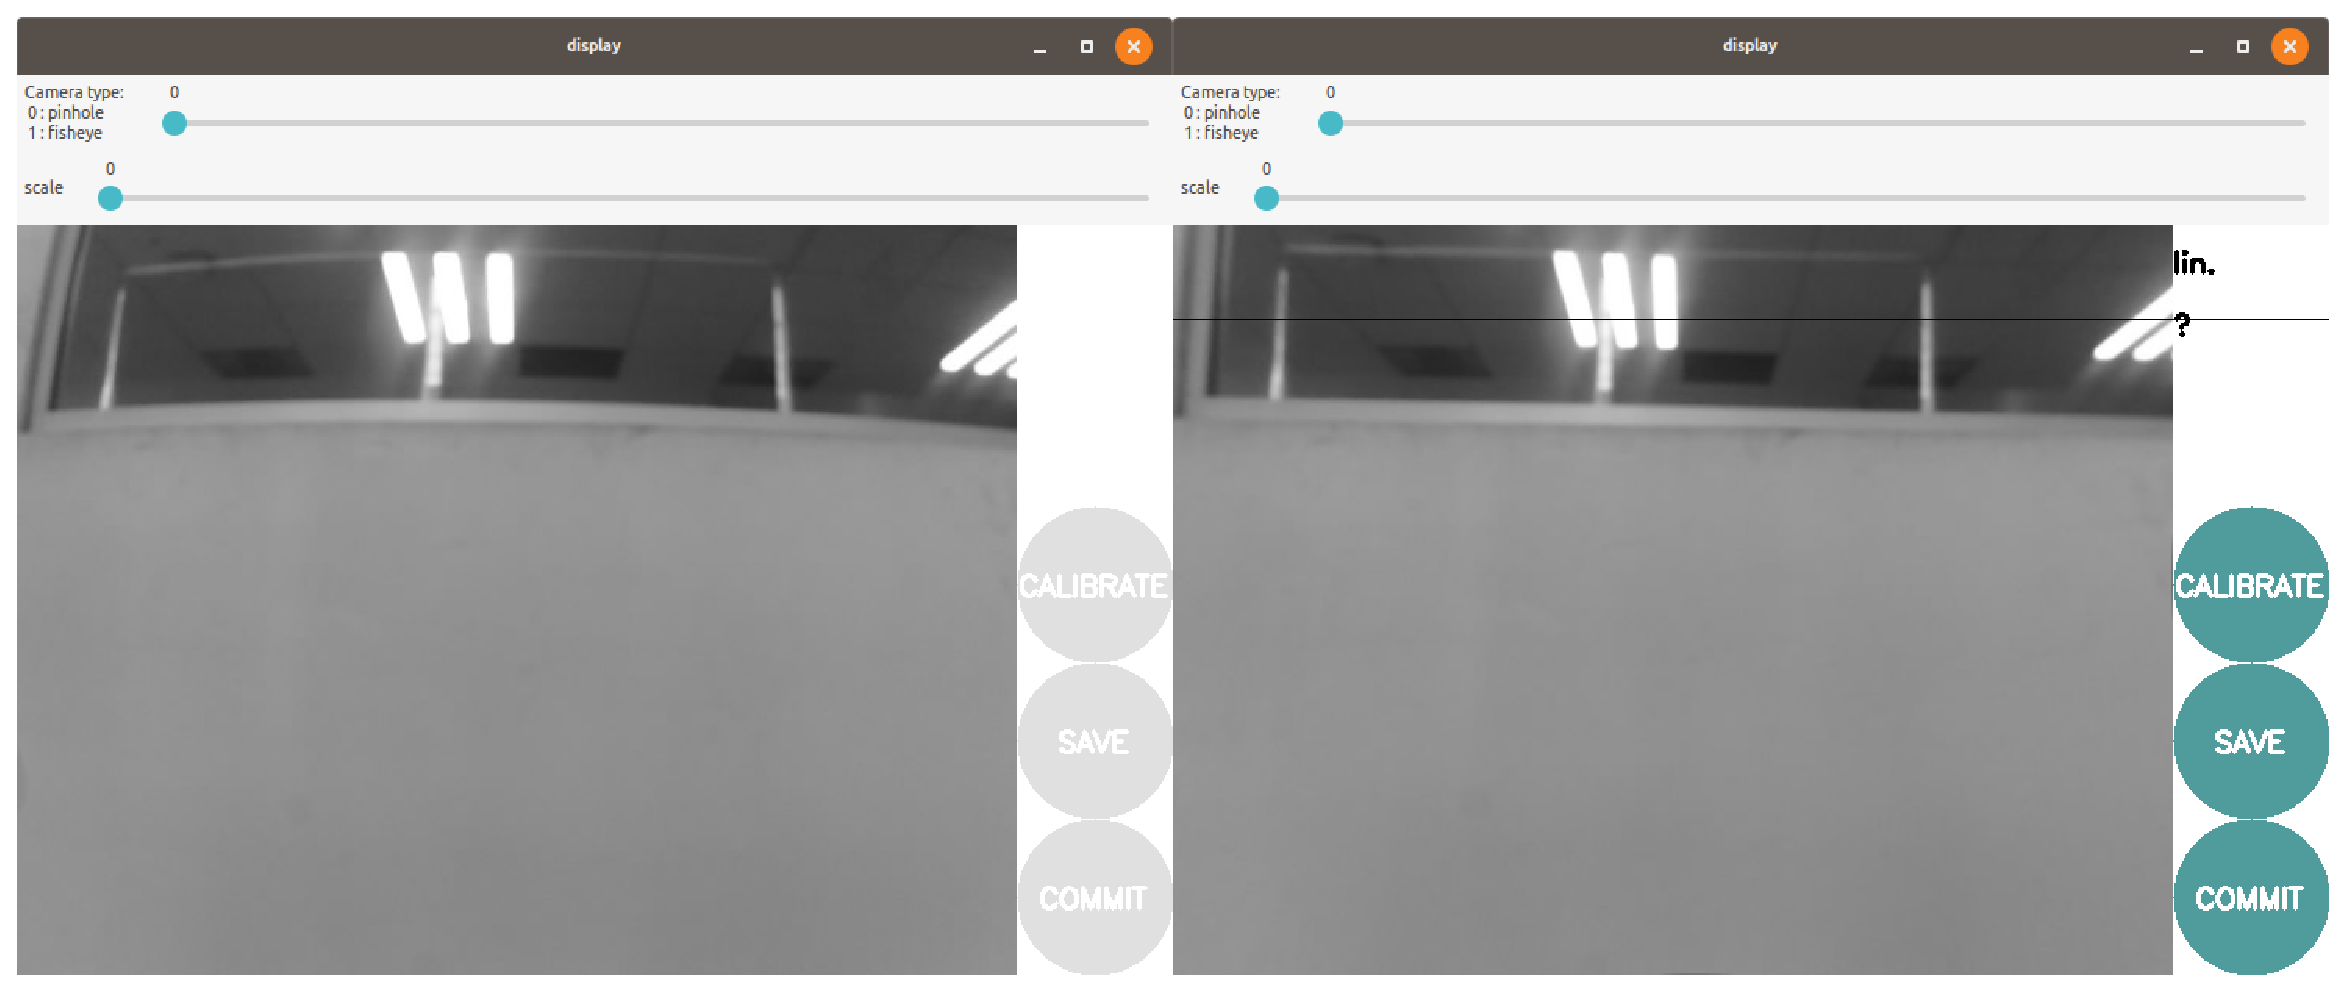
\includegraphics[width=0.7\textwidth]{Contenido/Cuerpo/Capitulo4/Fig10.eps}
	\captionof{figure}{Proceso de calibración utilizando un tablero de ajedrez}\label{Fig1}
\end{center}


% ---------------------------------------------------------------------------------------------------------
% *********************************************************************************************************
% *********************************************************************************************************
% ---------------------------------------------------------------------------------------------------------

\section{Espacio de color}
Como se puede apreciar en el algoritmo general, el paso 5 es el cambio de espacio de color
de RGB a HSV, además ya sabemos el porque es mejor generar colores partiendo del
modelo HSV. Así que lo que ahora sigue es la implementación en código y las pruebas
que se hicieron para tener un rango de colores y así tener una base de datos a la
cual recurriremos después.\\
El siguiente diagrama muestra el flujo que el programa 2(ver apéndice A) siguió para
el cambio de espacio de color.
\begin{center}
	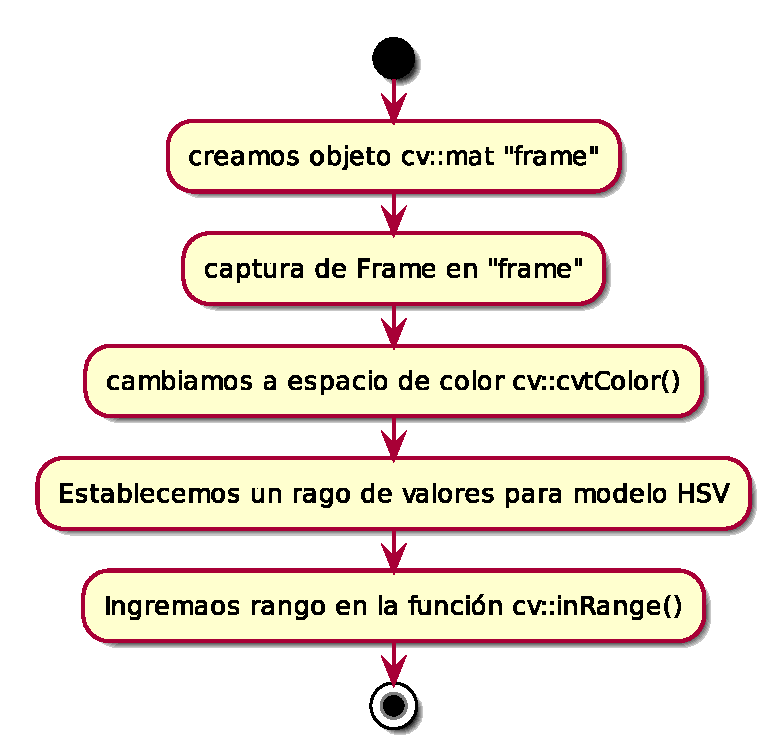
\includegraphics[width=0.5\textwidth]{Contenido/Cuerpo/Capitulo4/color.eps}
	\captionof{figure}{Diagrama de flujo para cambio de espacio de color}\label{color}
\end{center}
Empezamos con la función definida que nos dan las librerías de opencv para transformar
de RGB a HSV.
\begin{example}[label={ex:serie}]{cvtColor()}
	\textcolor{Mulberry}{void} \textcolor{RoyalBlue}{cv::cvtColor(}\textcolor{BurntOrange}{Mat}
	\textcolor{Mulberry}{\&}\textcolor{Bittersweet}{\_src}, \textcolor{BurntOrange}{Mat} \textcolor{Mulberry}{\&}\textcolor{Bittersweet}{dst}
	,\textcolor{Mulberry}{int} \textcolor{Bittersweet}{code}, \textcolor{Mulberry}{int} \textcolor{Bittersweet}{dstCn}
	\textcolor{RoyalBlue}{)}
\end{example}
Donde
\begin{itemize}
	\item \textbf{src}: Imagen de entrada de 8 bits sin signo
	\item \textbf{sdt}: Imagen de salida del mismo tamaño y profundidad que src.
	\item \textbf{code}: Código de conversión de espacio de color en este caso es \\COLOR\_BGR2HSV.
	\item \textbf{dstCn}: Número de canales en la imagen de destino; si el parámetro es 0, el
	      número de canales se deriva automáticamente de src y código.
\end{itemize}
El formato de color predeterminado en OpenCV a menudo se denomina RGB, pero en realidad
es BGR (los bytes se invierten). Entonces, el primer byte en una imagen en color estándar
(24 bits) será un componente azul de 8 bits, el segundo byte será verde y el tercer
byte será rojo. El cuarto, quinto y sexto bytes serían el segundo píxel (Azul, luego
Verde, luego Rojo), y así sucesivamente.
\begin{center}
	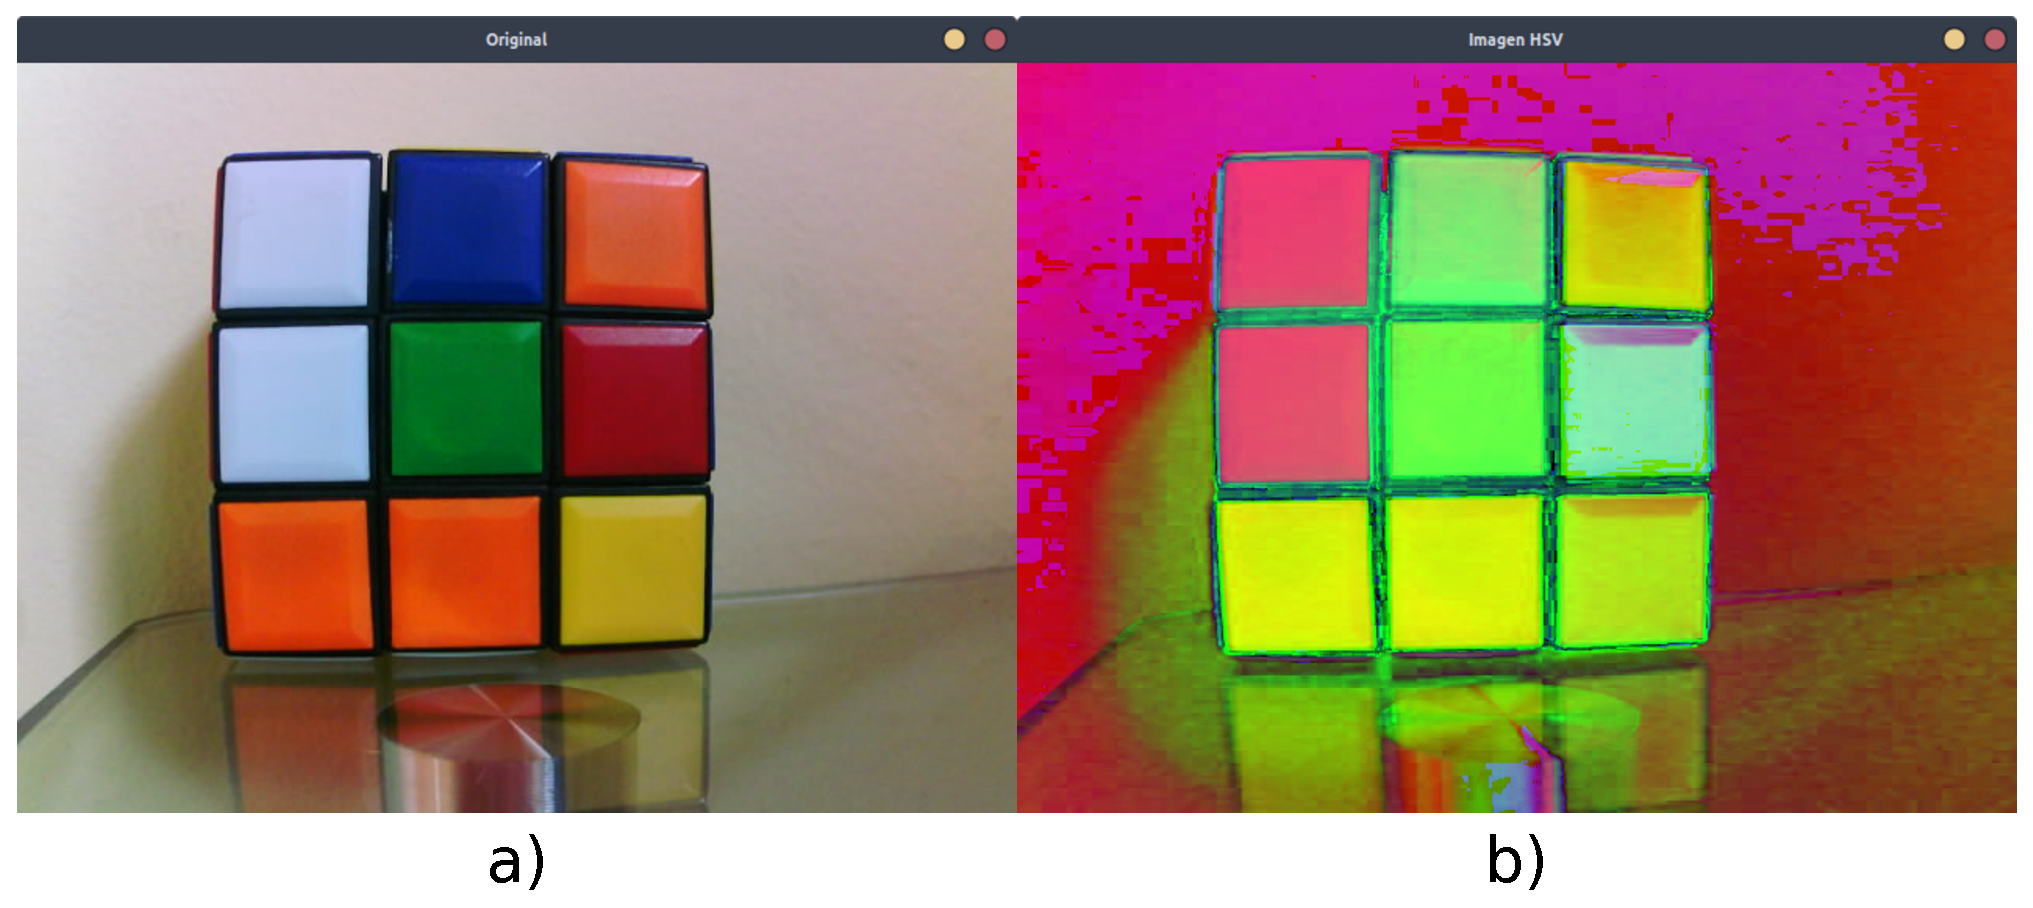
\includegraphics[width=0.9\textwidth]{Contenido/Cuerpo/Capitulo4/Fig2.eps}
	\captionof{figure}{a)Imagen RGB; b) Imagen HSV}\label{Fig6}
\end{center}
En la figura anterior podemos apreciar el cambio del espacio de color, en b) tenemos el resultado de aplicar la función cvtColor
con el código COLOR\_BGR2HSV, que podemos dividir a su vez en 3 canales, H$\arrowvert$Hue, S$\arrowvert$Saturation y
V$\arrowvert$Value.
\begin{center}
	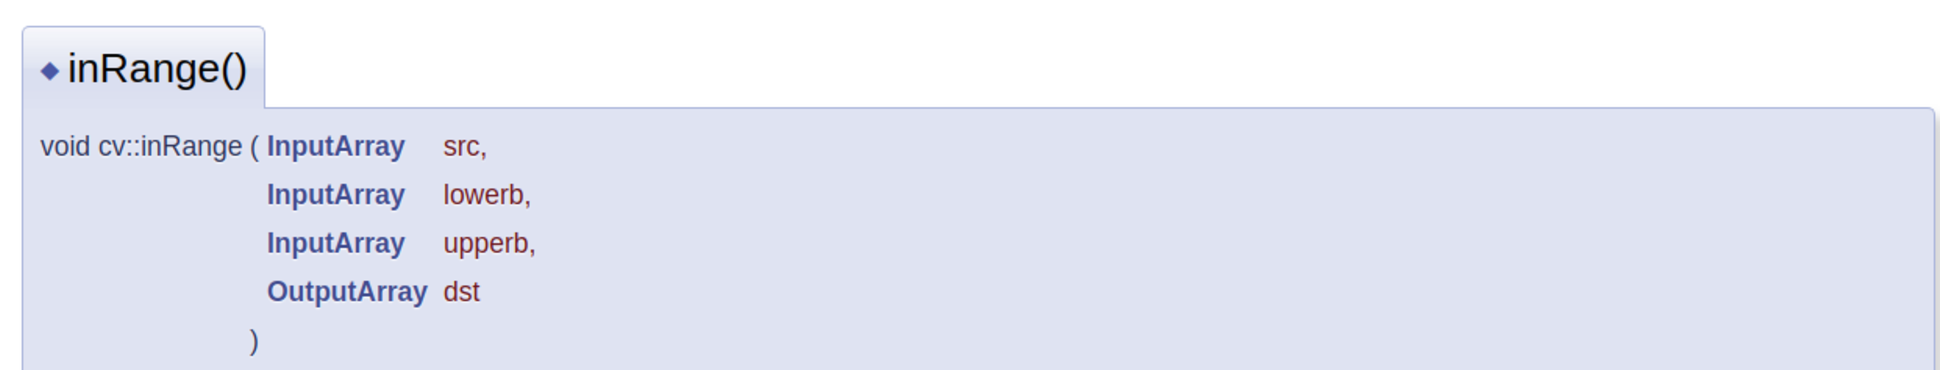
\includegraphics[width=0.9\textwidth]{Contenido/Cuerpo/Capitulo4/Fig3.eps}
	\captionof{figure}{Espacio de color HSV, a)Hue; b)Saturation; c)Value}\label{Fig6}
\end{center}

Ahora pasamos a la función que acota el color que deseemos, esta es la llamada inRange()
\begin{example}[label={ex:serie}]{inRange()}
	\textcolor{Mulberry}{void} \textcolor{RoyalBlue}{cv::cvtColor(}\textcolor{BurntOrange}{Mat}
	\textcolor{Mulberry}{\&}\textcolor{Bittersweet}{src}, \textcolor{BurntOrange}{Mat} \textcolor{Mulberry}{\&}\textcolor{Bittersweet}{lowerb},
	\textcolor{BurntOrange}{Mat} \textcolor{Mulberry}{\&}\textcolor{Bittersweet}{upperb},
	\textcolor{BurntOrange}{Mat} \textcolor{Mulberry}{\&}\textcolor{Bittersweet}{dst}
	\textcolor{RoyalBlue}{)}
\end{example}
Donde
\begin{itemize}
	\item \textbf{src} primera matriz de entrada.
	\item \textbf{lowerb} matriz de límite inferior o un escalar.
	\item \textbf{upper}  matriz de límite superior o un escalar.
	\item \textbf{dst} Conjunto de salida dst del mismo tamaño que src y tipo CV\_8U.
\end{itemize}
Debido a que no hay un solo color azul o rojo, etc, si no más bien un rango que cubre
la gama de azules, amarillo, naranja, etc. Por esa razón se hicieron pruebas para
determinar los valores HSV que corresponden a los siguientes colores: Amarillo, Azul,
Rojo, Verde y Naranja y de esta manera a la hora de seguir un objetivo de dado color
el sistema no tenga problemas en reconocer esa gama de color.\\
La siguiente figura ilustra una gama de colores que va desde el rojo al azul, donde la
tarea es obtener un conjunto de imagenes que correspondan a un sector de la misma.
\begin{center}
	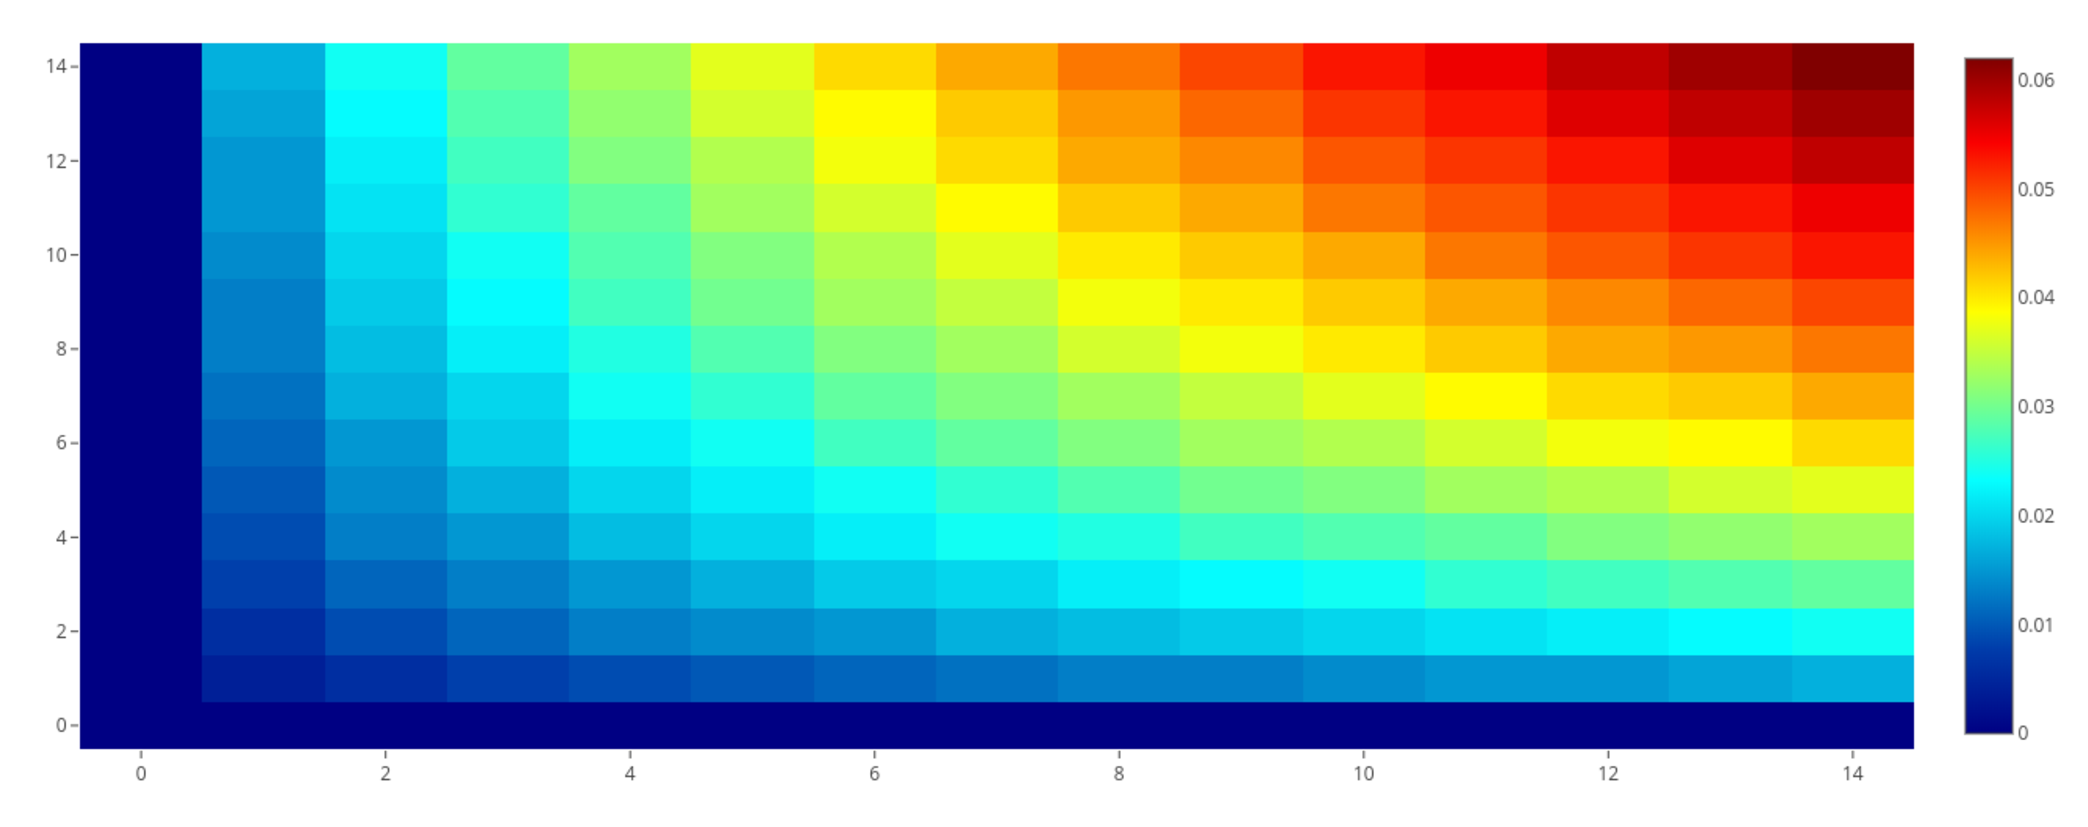
\includegraphics[width=0.6\textwidth]{Contenido/Cuerpo/Capitulo4/Fig4.eps}
	\captionof{figure}{Espectro de colores}\label{Fig6}
\end{center}
De donde apartir del código 2 se obtuvieron los siguientes resultados.
\begin{center}
	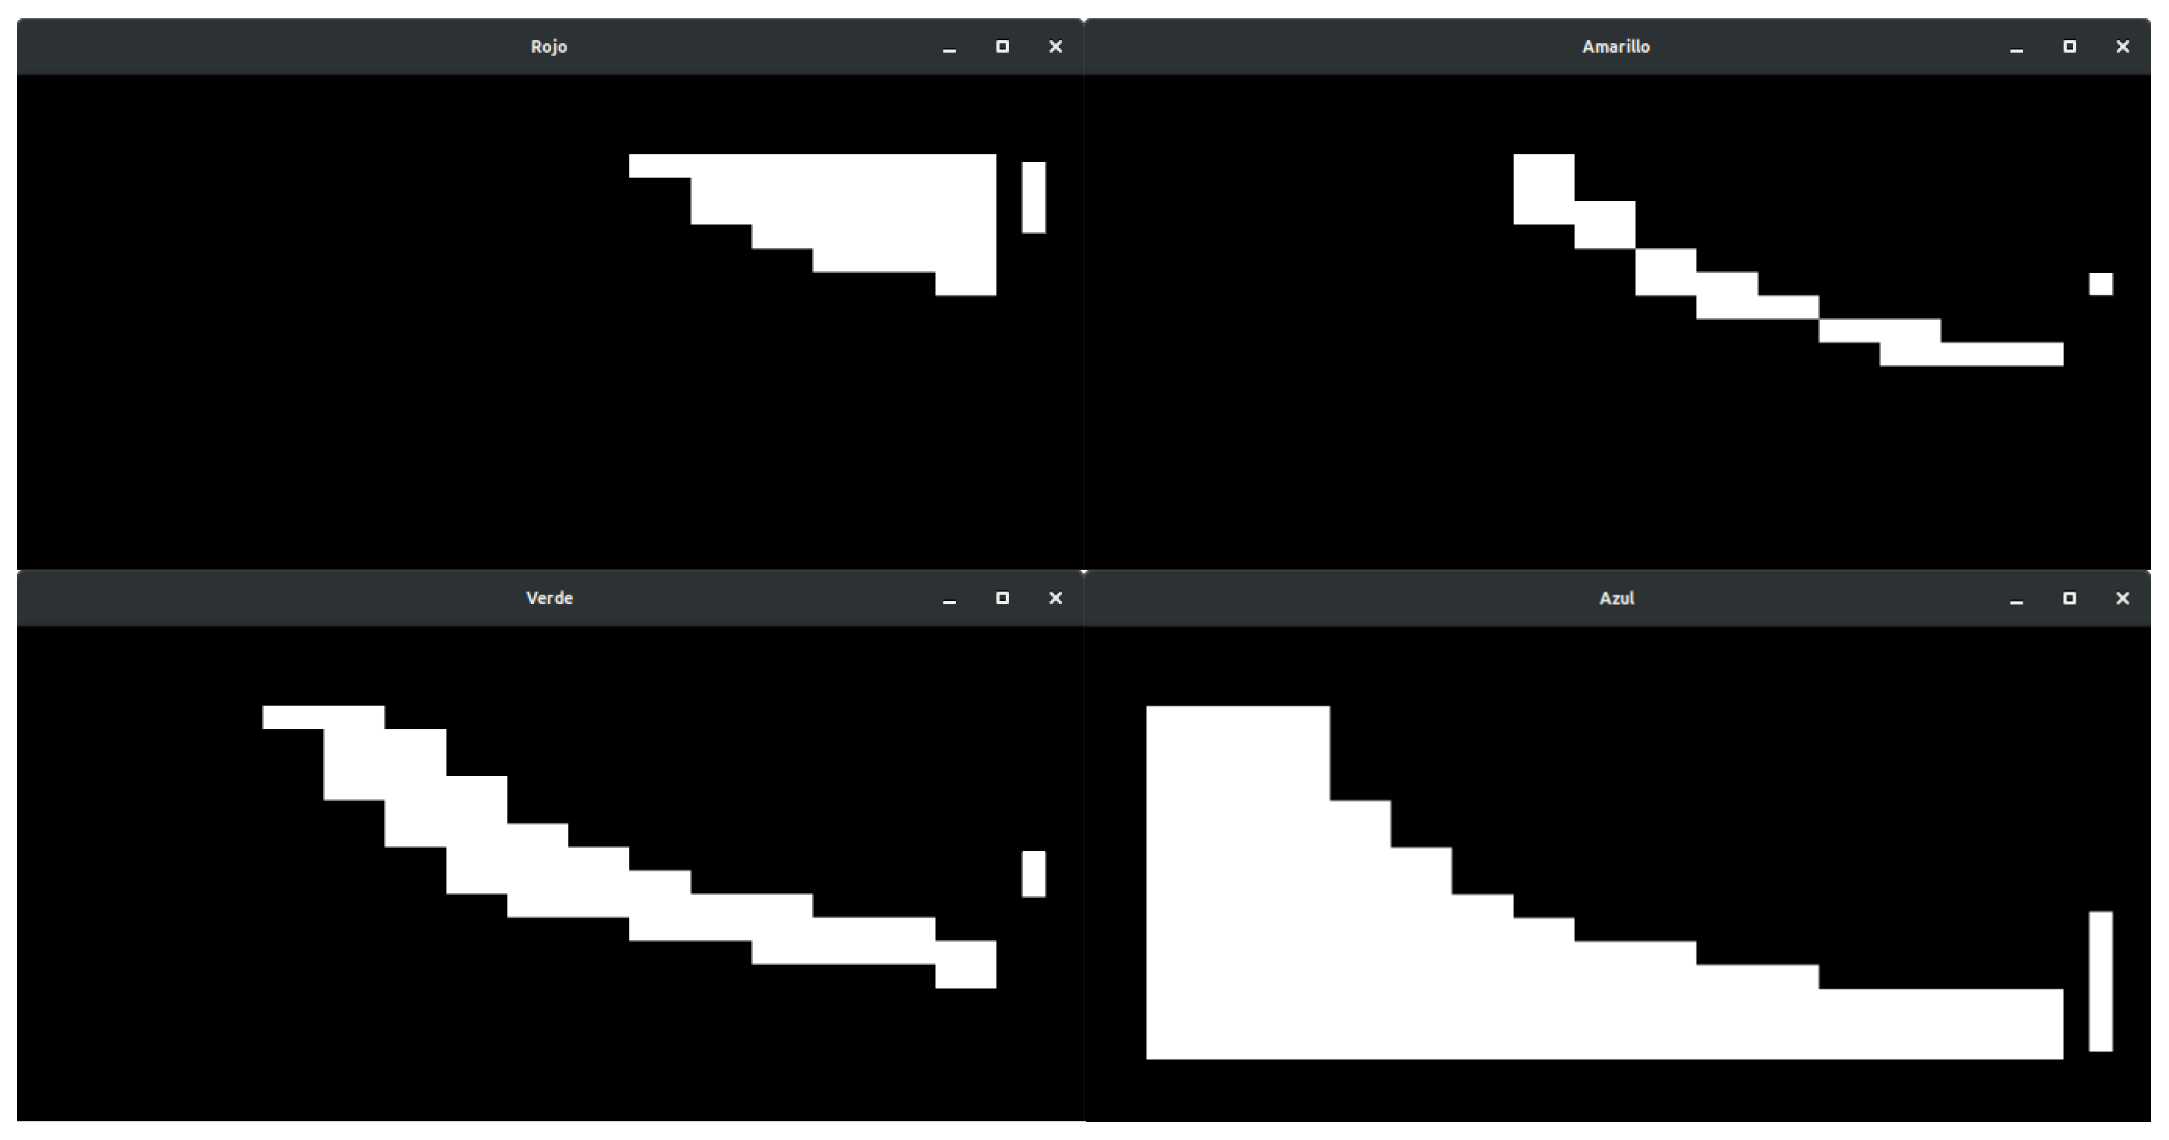
\includegraphics[width=0.6\textwidth]{Contenido/Cuerpo/Capitulo4/Fig5.eps}
	\captionof{figure}{Separación de colores}\label{Fig6}
\end{center}
En la figura 4.9 se aprecia la separación en 4 colores; Rojo, Amarillo, Verde y Azul.
con los siguientes rangos de valores.\\
\begin{table}[ht]
	\begin{center}
		\caption{Valores para cada rango de color}
		\begin{tabular}[t]{lcccccc}
			\hline
			         & H$_{min}$ & H$_{max}$ & S$_{min}$ & S$_{max}$ & V$_{min}$ & V$_{max}$ \\
			\hline
			Rojo     & 0         & 10        & 100       & 255       & 100       & 255       \\
			Amarillo & 25        & 35        & 50        & 255       & 50        & 255       \\
			Verde    & 35        & 75        & 100       & 255       & 100       & 255       \\
			Azul     & 75        & 130       & 55        & 255       & 55        & 255       \\
			\hline
		\end{tabular}
	\end{center}
\end{table}\\
A manera de tener una mejor visualización de los resultados, la siguiente figura concatena
cada segmento de color y le asigna un color plano a cada uno.
\begin{center}
	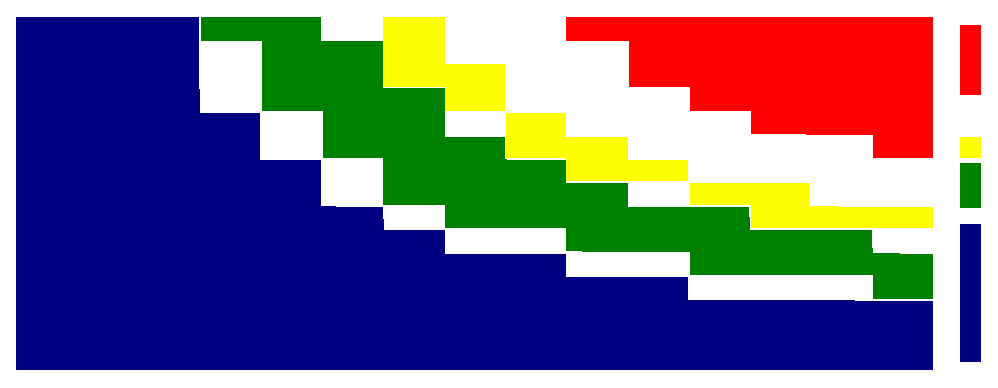
\includegraphics[width=0.6\textwidth]{Contenido/Cuerpo/Capitulo4/Fig6.eps}
	\captionof{figure}{Separación de colores}\label{Fig6}
\end{center}

\subsection{Pruebas de campo}
Una vez obtenido los valores aproximados de 4 rango de color, lo siguiente fue probar
dichos valores en una imagen captada por la cámara.\\
Las pruebas se hicieron con luz emitida por un foco, y con poca interacción con la
energía solar, probando primero el rango de color azul.
\begin{center}
	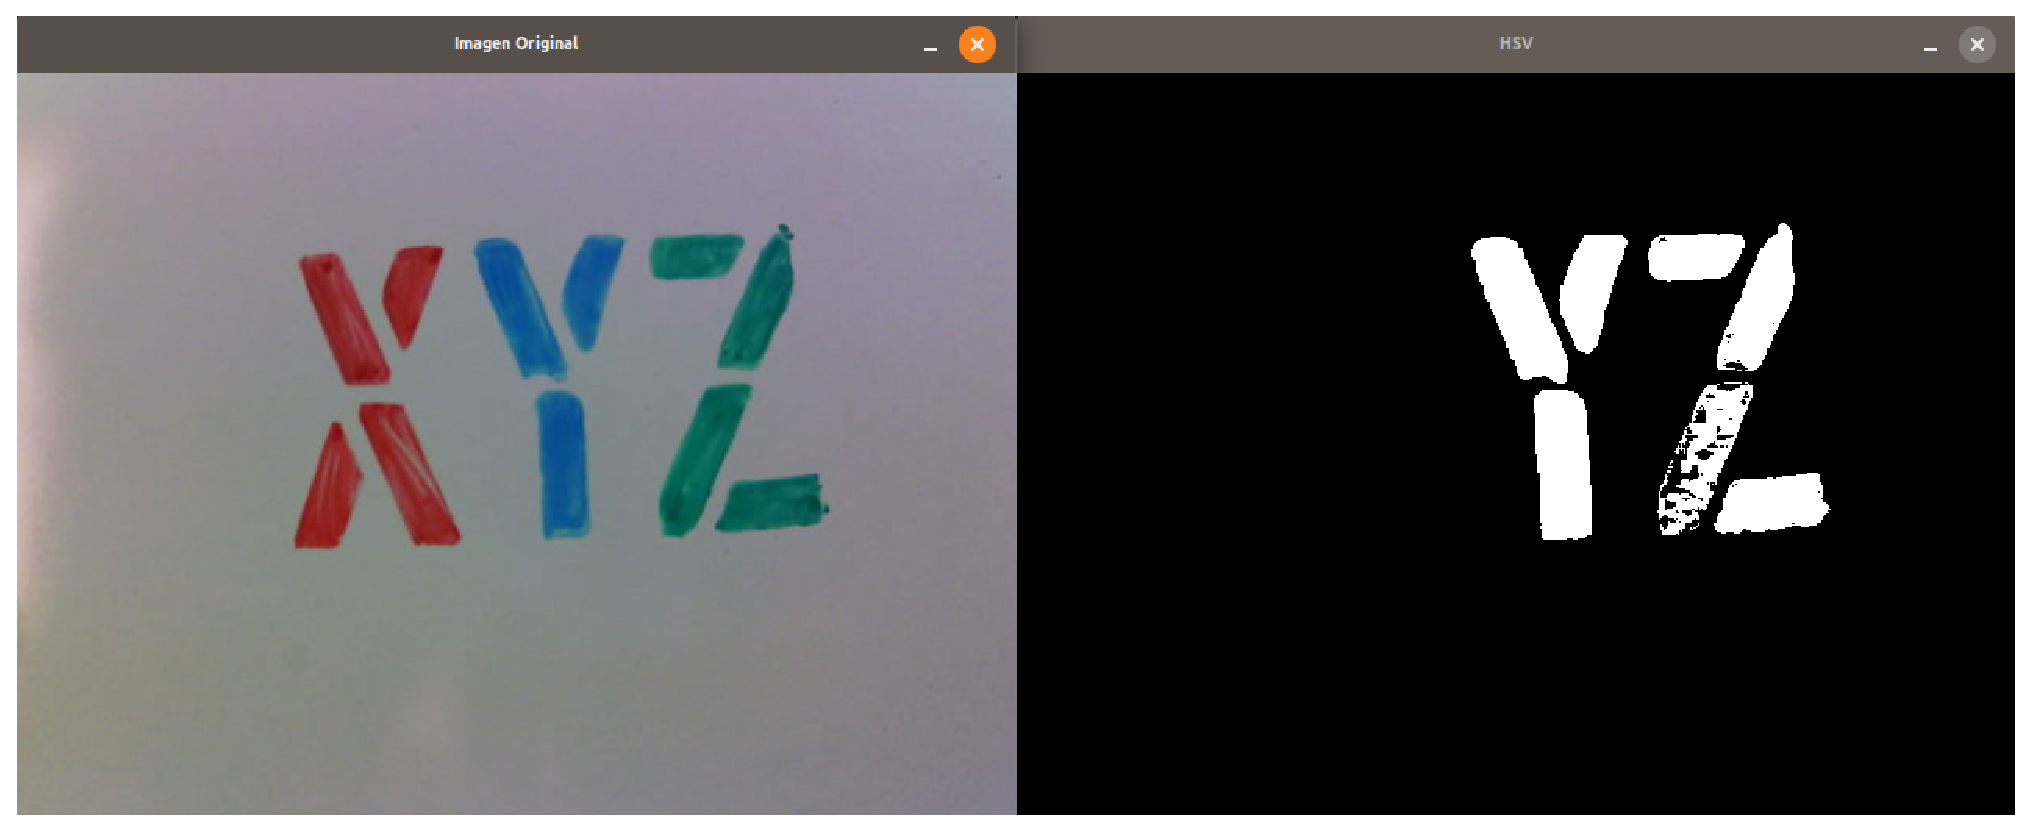
\includegraphics[width=0.8\textwidth]{Contenido/Cuerpo/Capitulo4/Fig7.eps}
	\captionof{figure}{Separación de color azul}\label{Fig7}
\end{center}
Como se puede observar en la figura anterior gran parte del color verde esta encapsulada
en lo que deberia ser únicamente color azul, esto debido aunque en las pruebas iniciales
no se consideró la variación de iluminación en el entorno, por lo que reajustar los
valores se hace una tarea necesaria. Aunque los primero valores de la tabla 4.1
no son exactos, nos sirven para tener una referencia de donde empezar a trabajar.\\
Una vez corregido el resultado del color azul se muestra en la siguiente figura.
\begin{center}
	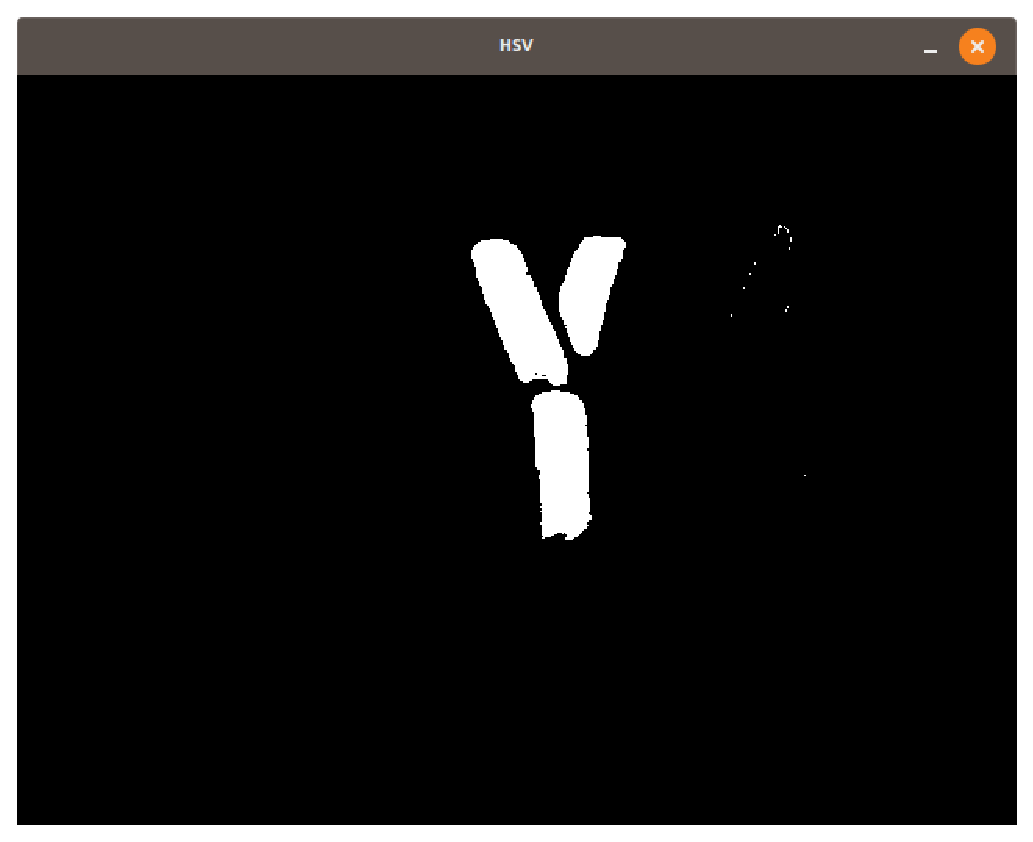
\includegraphics[width=0.5\textwidth]{Contenido/Cuerpo/Capitulo4/Fig9.eps}
	\captionof{figure}{Separación de colore azul}\label{Fig8}
\end{center}
Que al final tenemos la separación de los colores primarios como se muestra en la siguiente
figura, donde se debe mencionar uno de los principales problemas que presenta este algoritmo.
\begin{center}
	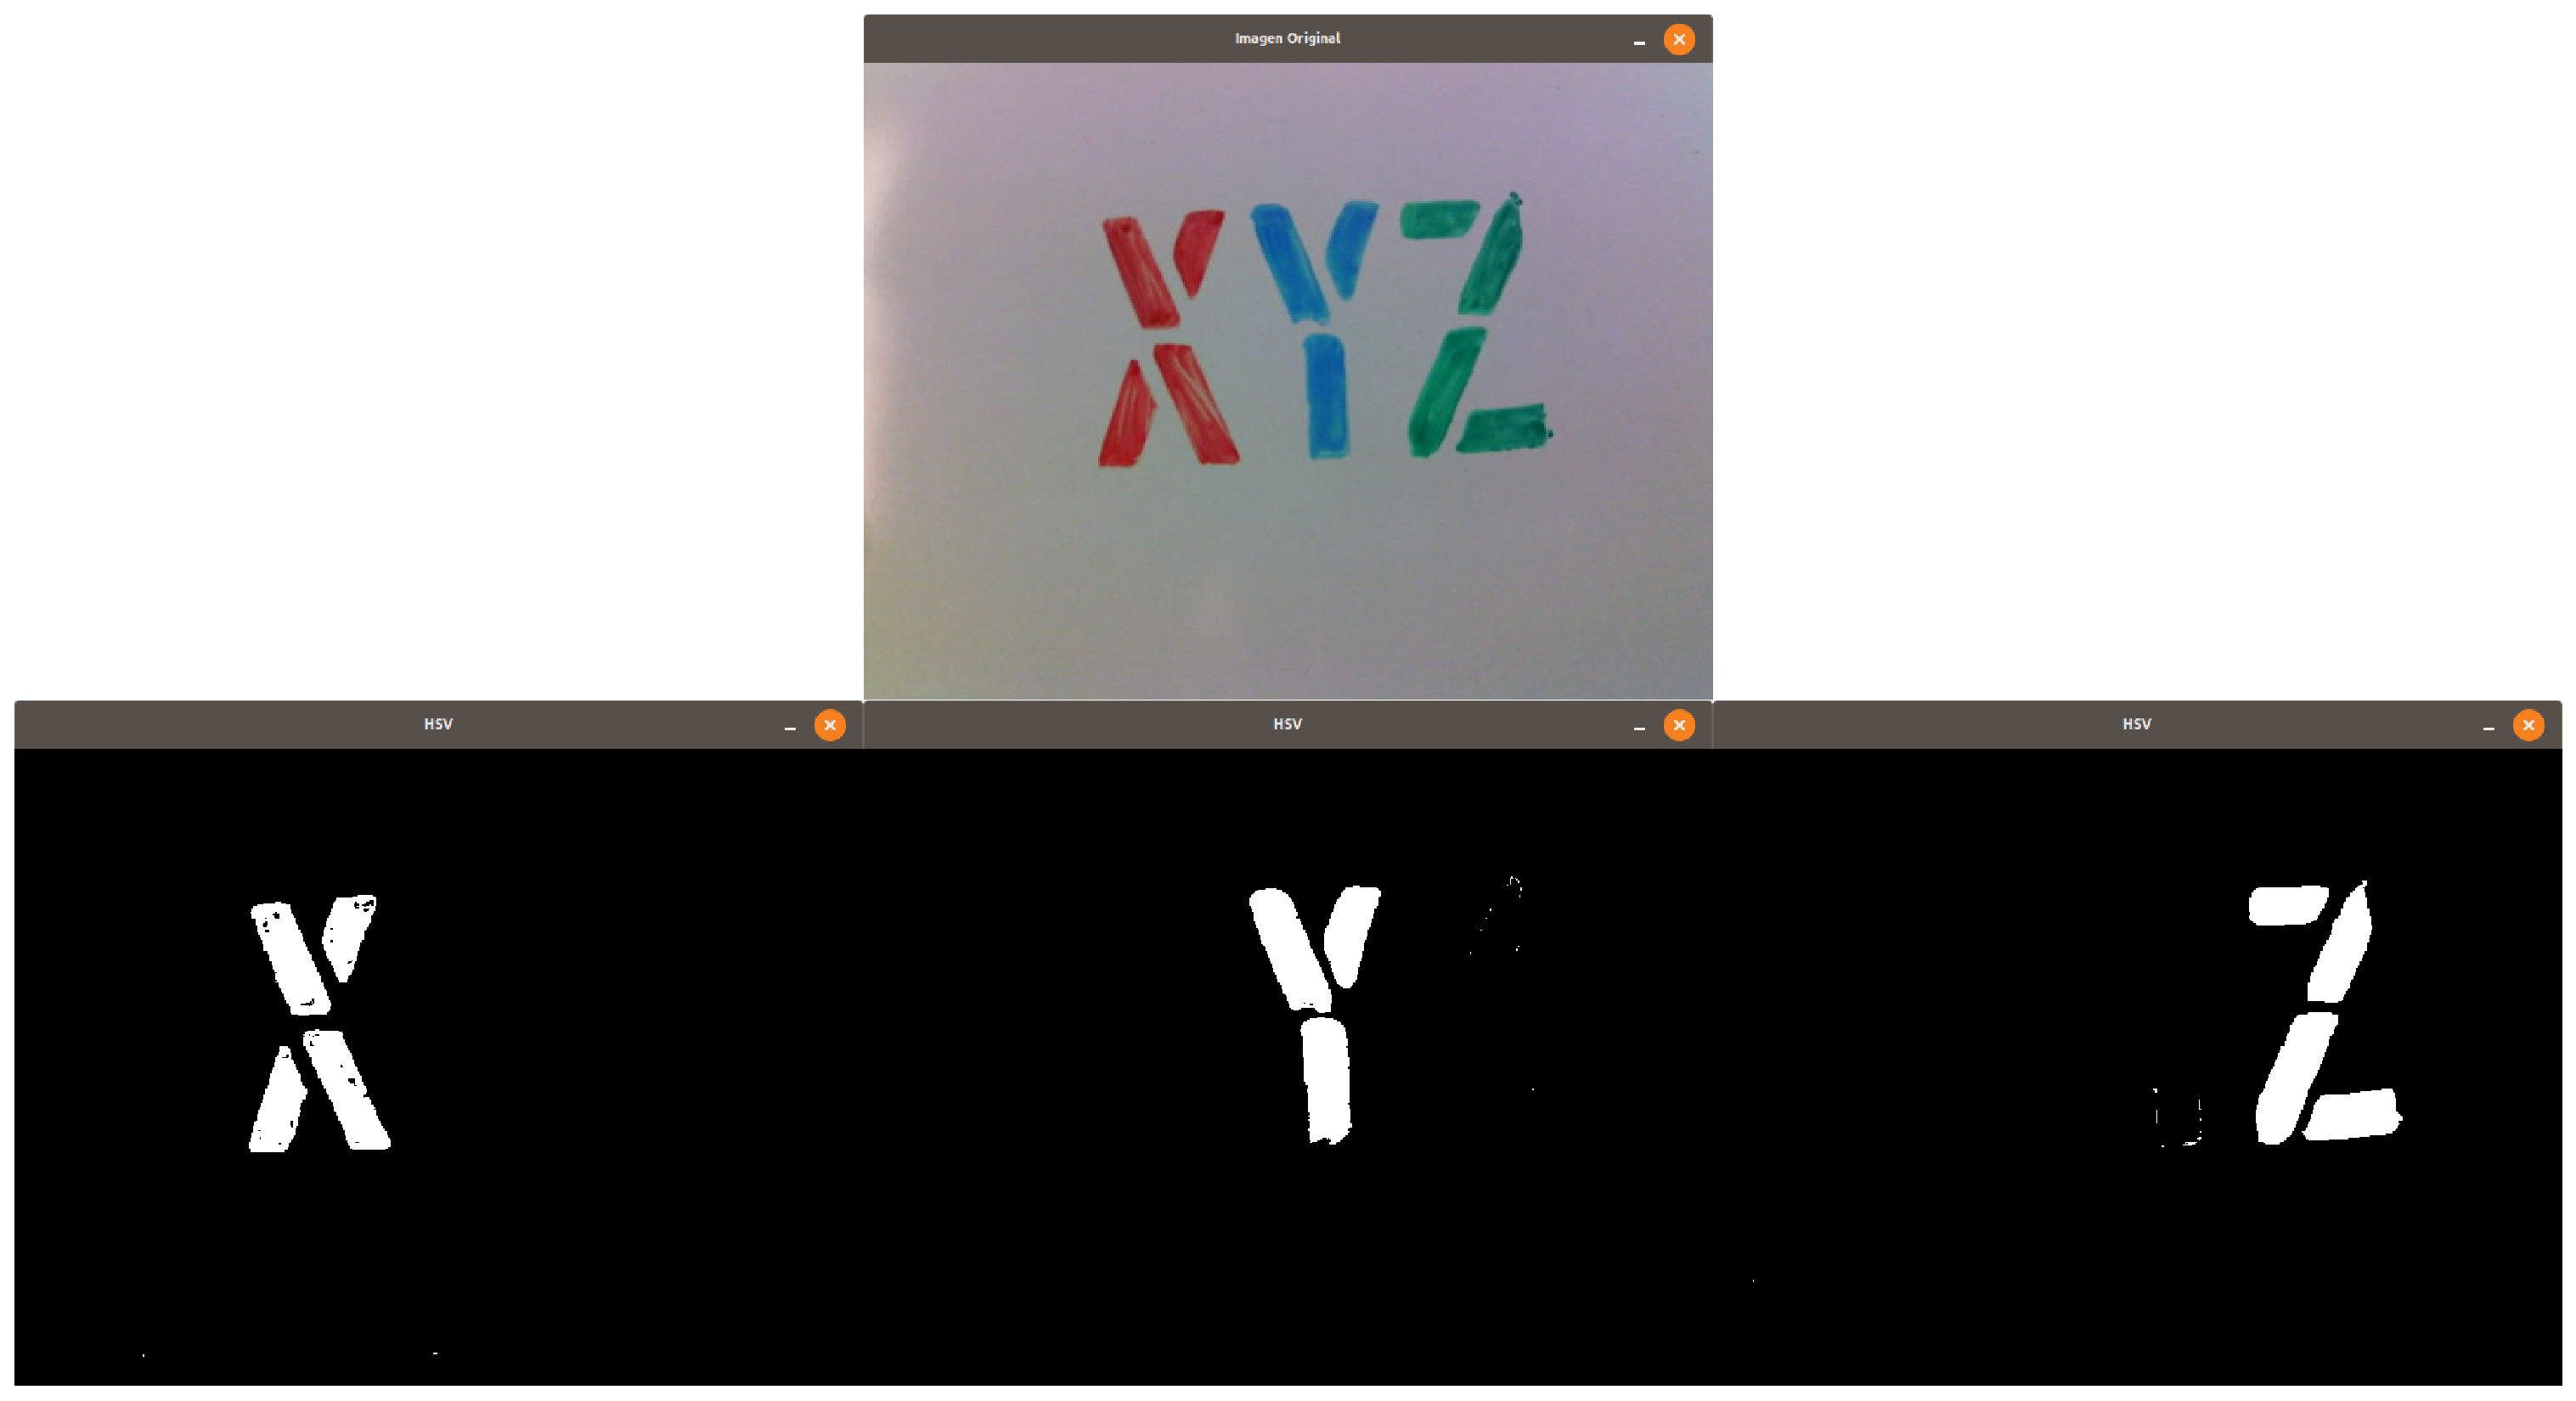
\includegraphics[width=0.5\textwidth]{Contenido/Cuerpo/Capitulo4/Fig8.eps}
	\captionof{figure}{Separación de colores RGB utilizando el modelo HSV}\label{Fig9}
\end{center}
El problema es que debido a que no tenemos un sensor que mida la intensidad de luminosidad
nuestro rango de los valores S y V van a cambiar dependiendo del entorno en el que este la cámara
es decir, que si hay alguna sombra que haga pensar al algoritmo que el color es verde, cuando en
realidad es azul.
Para las pruebas anteriores se obtuvieron de resultado los siguiente valores.\\
\begin{table}[ht]
	\begin{center}
		\caption{Valores para cada rango de color en un ambiente iluminado por energía eléctrica}
		\begin{tabular}[t]{lcccccc}
			\hline
			         & H$_{min}$ & H$_{max}$ & S$_{min}$ & S$_{max}$ & V$_{min}$ & V$_{max}$ \\
			\hline
			Rojo     & 0         & 10        & 70        & 255       & 70        & 255       \\
			Amarillo & 25        & 35        & 50        & 255       & 50        & 255       \\
			Verde    & 35        & 90        & 55        & 255       & 55        & 255       \\
			Azul     & 95        & 130       & 55        & 255       & 55        & 255       \\
			\hline
		\end{tabular}
	\end{center}
\end{table}\\
Otro problema que es palpable de ver es la captación de ruido, en las dos figuras anteriores
hay presencia de pequeño ruido tanto fuera como dentro de las letras. Esto se puede solucionar
agregando un par de filtros básicos, los llamadas opening y closing.

% ---------------------------------------------------------------------------------------------------------
% *********************************************************************************************************
% *********************************************************************************************************
% ---------------------------------------------------------------------------------------------------------
\section{Corrección de brillo}
Como se pudo observar en pruebas anteriores el rango que se asigna a cada color en el modelo HSV está
completamente ligado con la cantidad de iluminación de nuestra imagen, es por eso que predefinir
un conjunto de valores se hace una tarea complicada, una solución sería poner 3 barras de interfaz
para acomodar los valores de H S y V, lo cual sería una solución sencilla pero un poco tardada, ya que
el sistema tendrá que responder en tiempo real a los cambios de los valores antes descritos.\\
Otra posible solución es corregir el brillo por medio de la librería de OpenCV,
y de la misma manera poner una barra en la interfaz que ajuste el brillo de modo manual. Dicha solución
parece ser la mejor opción para este proyecto debido a que solo necesitamos mover un rango de valor y dejar
fijos los parámetros del espacio de color, esto, claro se tiene que hacer antes de transformar de RGB
a HSV.\\
El ajuste de brillo y saturación se da a partir de la siguiente expresión
\begin{equation}
	g(i,j) = \alpha * f(i,j) + \beta
\end{equation}
Donde $\alpha$ es el encargado de ajustar el contraste, mientras que $\beta$ se encarga del brillo.
Los valores de $\alpha$ van en el rango de 1 a 3, de tipo float y los de $\beta$ van de 0 a 100 de tipo entero.


Que visto desde los nodos de ROS quedaría así:
\begin{center}
	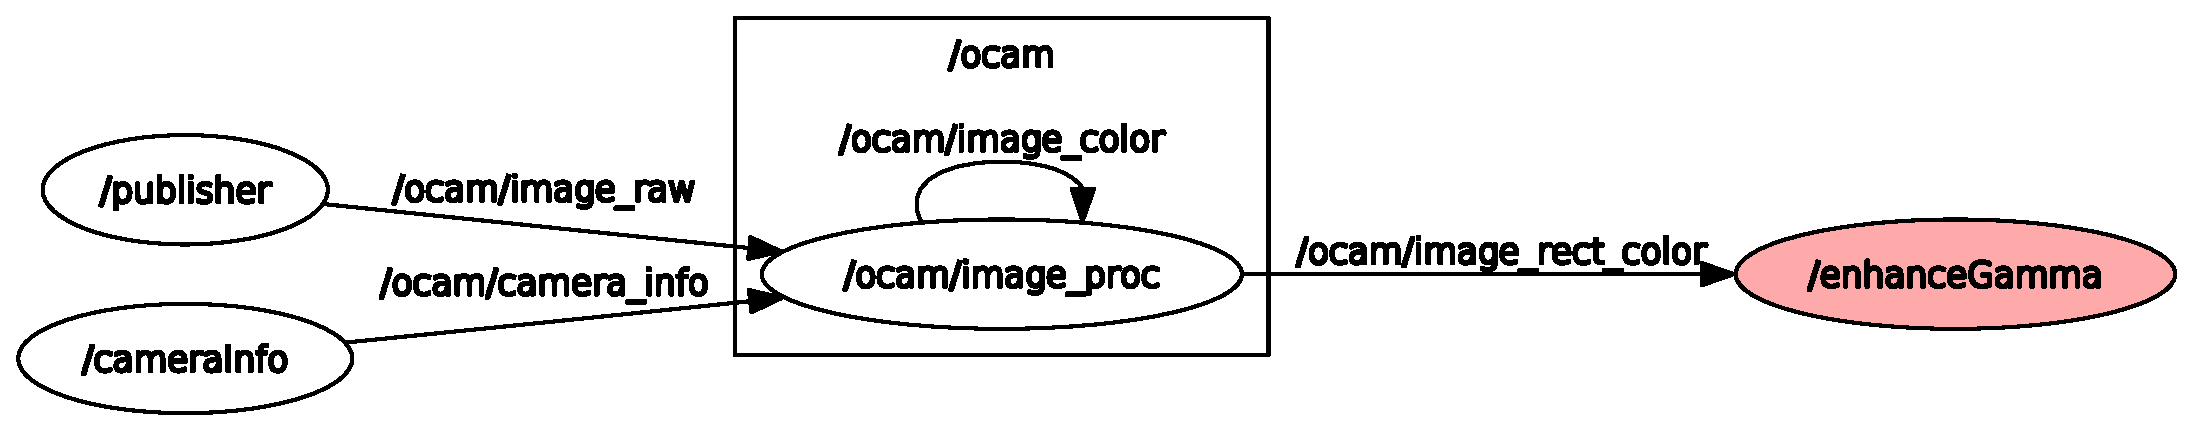
\includegraphics[width=0.65\textwidth]{Contenido/Cuerpo/Capitulo4/Fig14.eps}
	\captionof{figure}{Comunicación de nodos}\label{Fig9}
\end{center}
El nodo en rojo es el correspondiente a la etapa de correción, que se agrega a los nodos
publicador y calibrador.\\
Como pruba se utilizo un conjunto de letras de diferentes colores, impresas en papel blanco
\begin{center}
	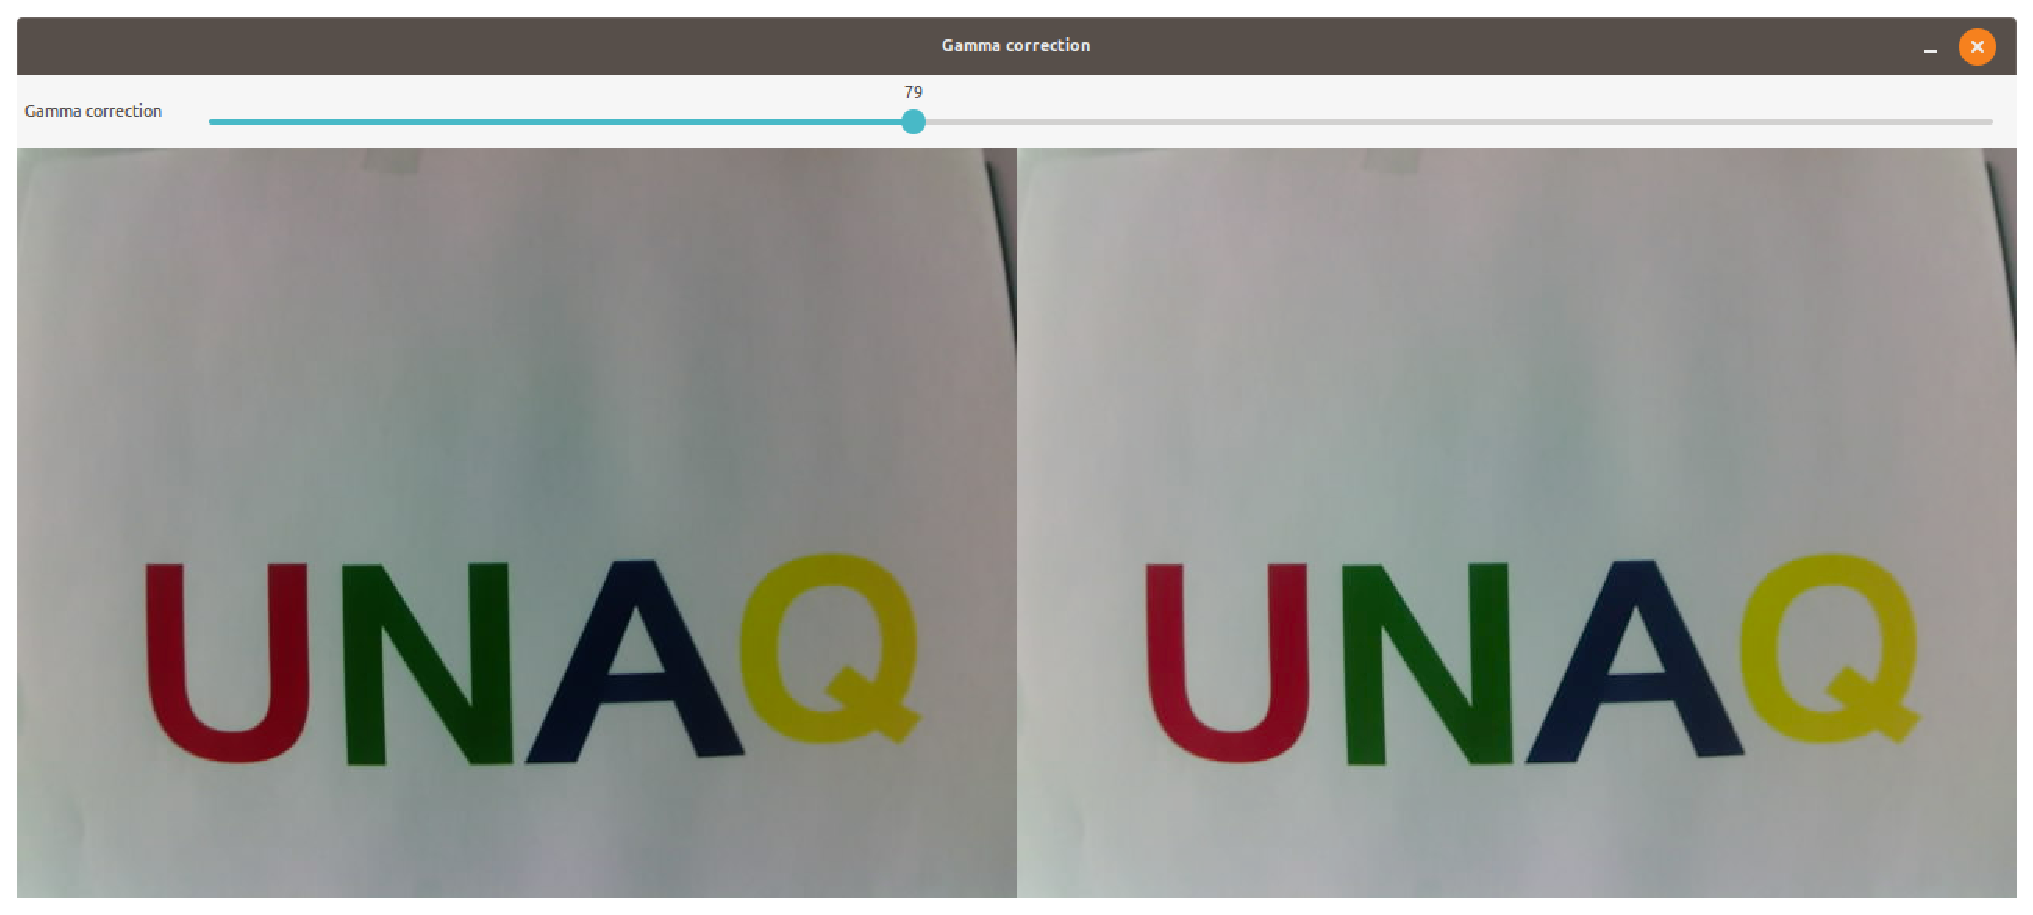
\includegraphics[width=0.65\textwidth]{Contenido/Cuerpo/Capitulo4/Fig13.eps}
	\captionof{figure}{correción de gamma, la imagen de la derecha es la corregida}\label{Fig9}
\end{center}
De la imagen anterior podemos observar dos cosas importantes, la primera es la barra de valores
que interactúan con el usuario, que va de 0 a 200 y es la correspondiente al valor de gamma. Y en
segundo claramente se percibe un realce de colores y como es que el fondo se ve más claro, que esto
ayuda de alguna manera a limpiar la imagen al no agregar ruido innecesario.

% ---------------------------------------------------------------------------------------------------------
% *********************************************************************************************************
% *********************************************************************************************************
% ---------------------------------------------------------------------------------------------------------

\section{Filtro morfologico}
Como vimos en la sección de HSV el entorno puede llegar a introducir a nuestra
imagen un poco de ruido por lo que es necesario aplicar técnicas de filtrado.\\
Las librerías de opencv proveen operadores morfológicos que nos ayudan a limpiar
nuestra imagen.
Dicho filtros son los que abordamos en el capitulo 1, opening y closing que nos ayudaran
a limpiar el objetivo por dentro y por fuera.
\begin{example}[label={ex:serie}]{Operación Morfologica}
	\textcolor{Mulberry}{void} \textcolor{RoyalBlue}{morphologyOperation(}\textcolor{BurntOrange}{Mat}
	\textcolor{Mulberry}{\&}\textcolor{Bittersweet}{\_Image}, \textcolor{BurntOrange}{Mat} \textcolor{Mulberry}{\&}\textcolor{Bittersweet}{Image\_}
	,\textcolor{Mulberry}{int} \textcolor{Bittersweet}{oper}, \textcolor{Mulberry}{int} \textcolor{Bittersweet}{size},
	\textcolor{Mulberry}{int} \textcolor{Bittersweet}{elemen}\textcolor{RoyalBlue}{)}
\end{example}
De la función anterior tenemos que:
\begin{itemize}
	\item \textbf{\_Image} es la imagen de entrada.
	\item \textbf{Image\_} es la imagen de salida
	\item \textbf{Oper} indica la operación Morfologica, 0 para opening y 1 para closing.
	\item \textbf{size} El tamaño del kernel.
	\item \textbf{elemn} La forma del kernel; 0 $\rightarrow$ Rectangular; 1 $\rightarrow$ Elipse y
	      2 $\rightarrow$ Cruz.
\end{itemize}
Los últimos dos parámetros son lo que se modificaron en las siguientes pruebas.
\begin{center}
	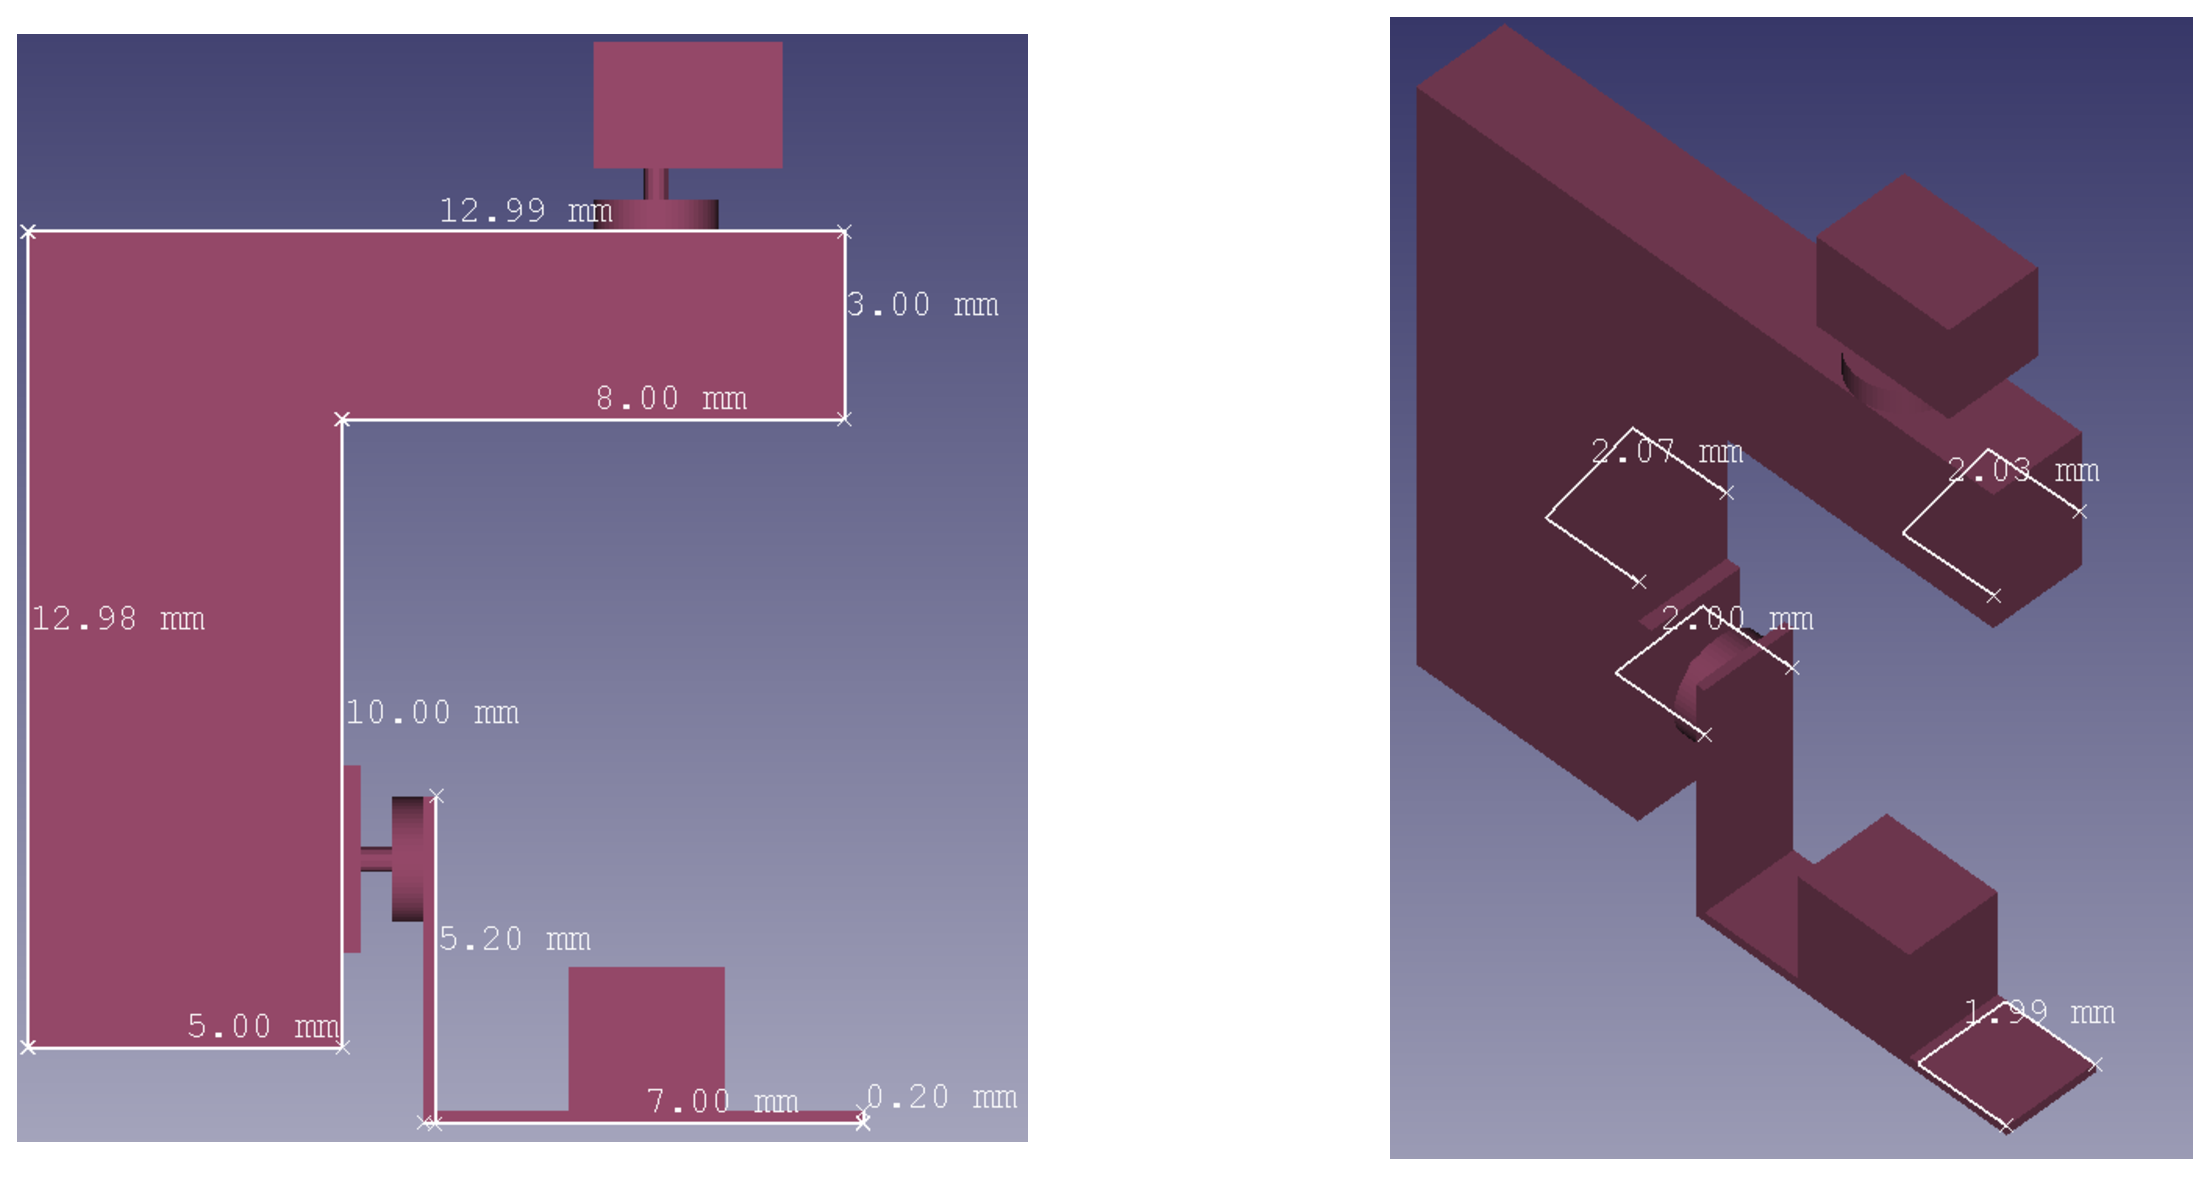
\includegraphics[width=0.6\textwidth]{Contenido/Cuerpo/Capitulo4/Fig16.eps}
	\captionof{figure}{A) Imagen original, B)Aplicación de flitros}\label{Fig9}
\end{center}
En la imagen anterior la aplicación del filtro se hizo con un kernel para el opening cuadrado y con un tamaño de 1.
Se puede observar que no hay un cambio significativo por lo que se decidió cambiar a un kernel cuadrado
de tamaño 3, la elección del kernel cuadrado es porque el objetivo tiene bordes de aproximadamente 90
grados.
\begin{center}
	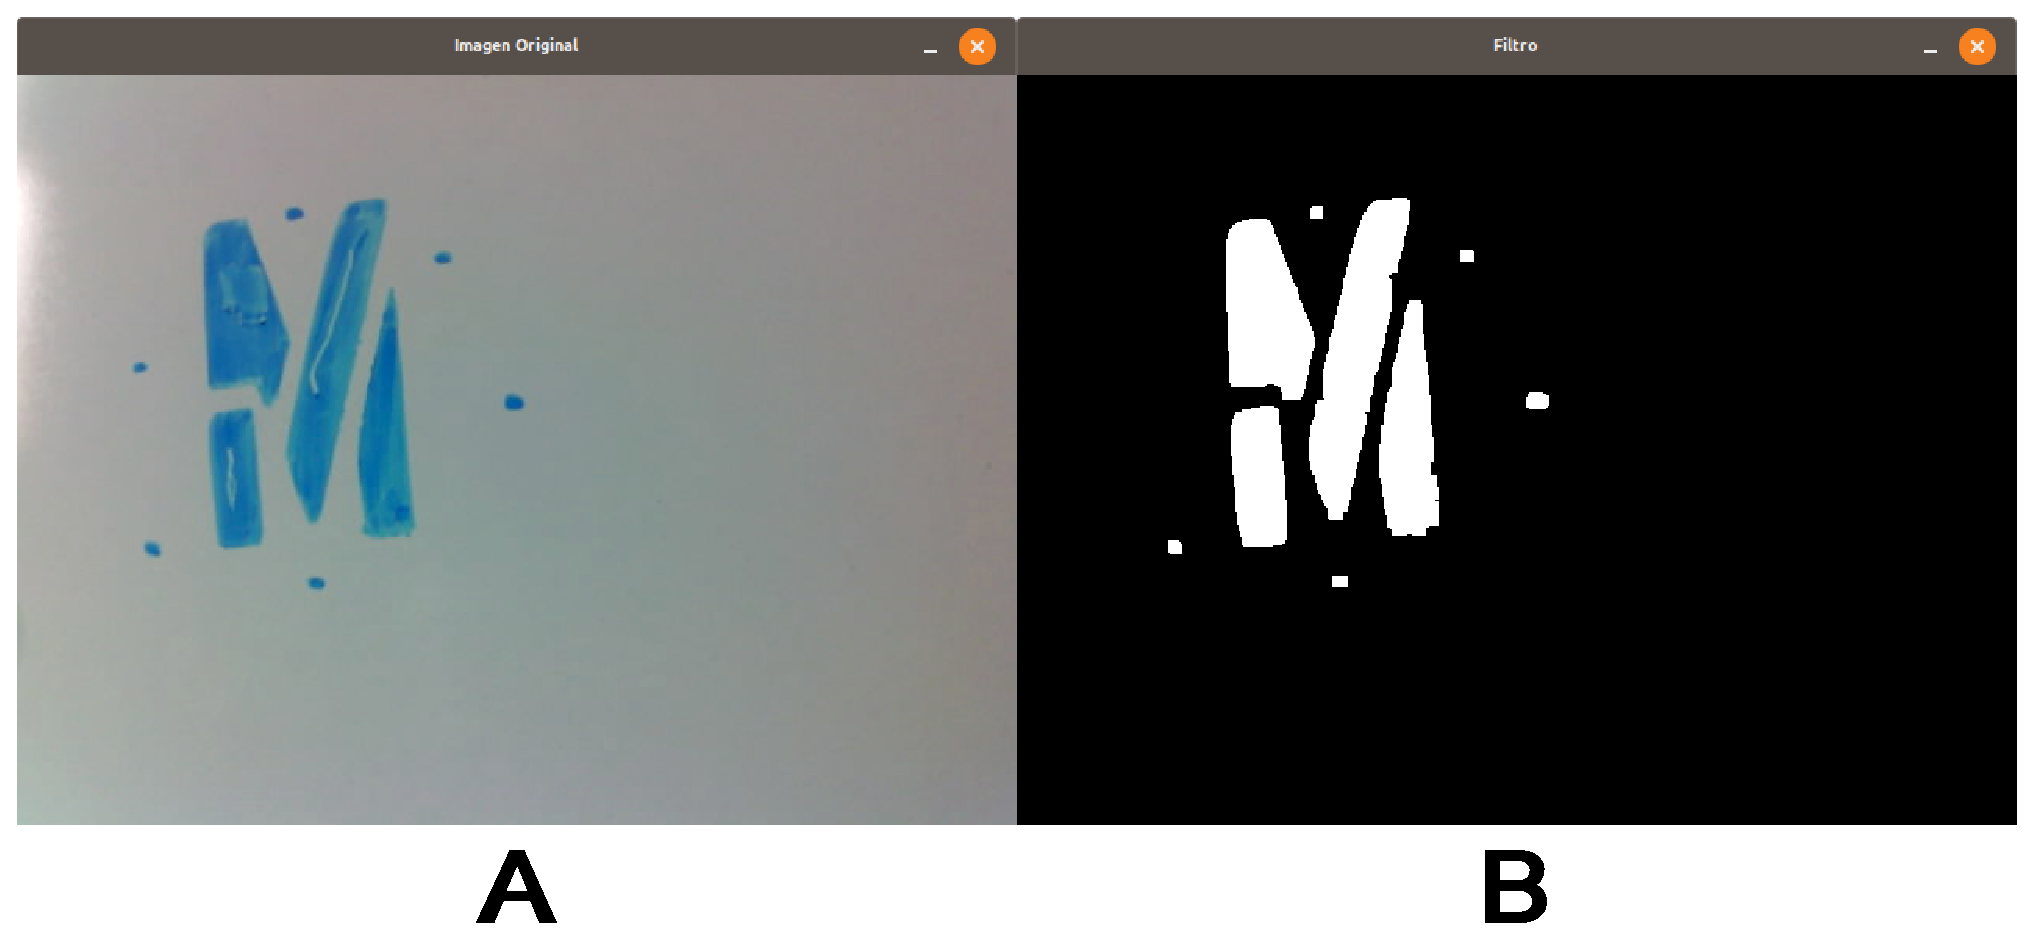
\includegraphics[width=0.6\textwidth]{Contenido/Cuerpo/Capitulo4/Fig17.eps}
	\captionof{figure}{A) Imagen original, B)Aplicación de flitros. Con size de 3}\label{Fig9}
\end{center}
Hubo ligeros cambios, solo desaparecieron algunos puntos que son ruido por lo que es conveniente aumentar
el parámetro \textbf{size}.
\begin{center}
	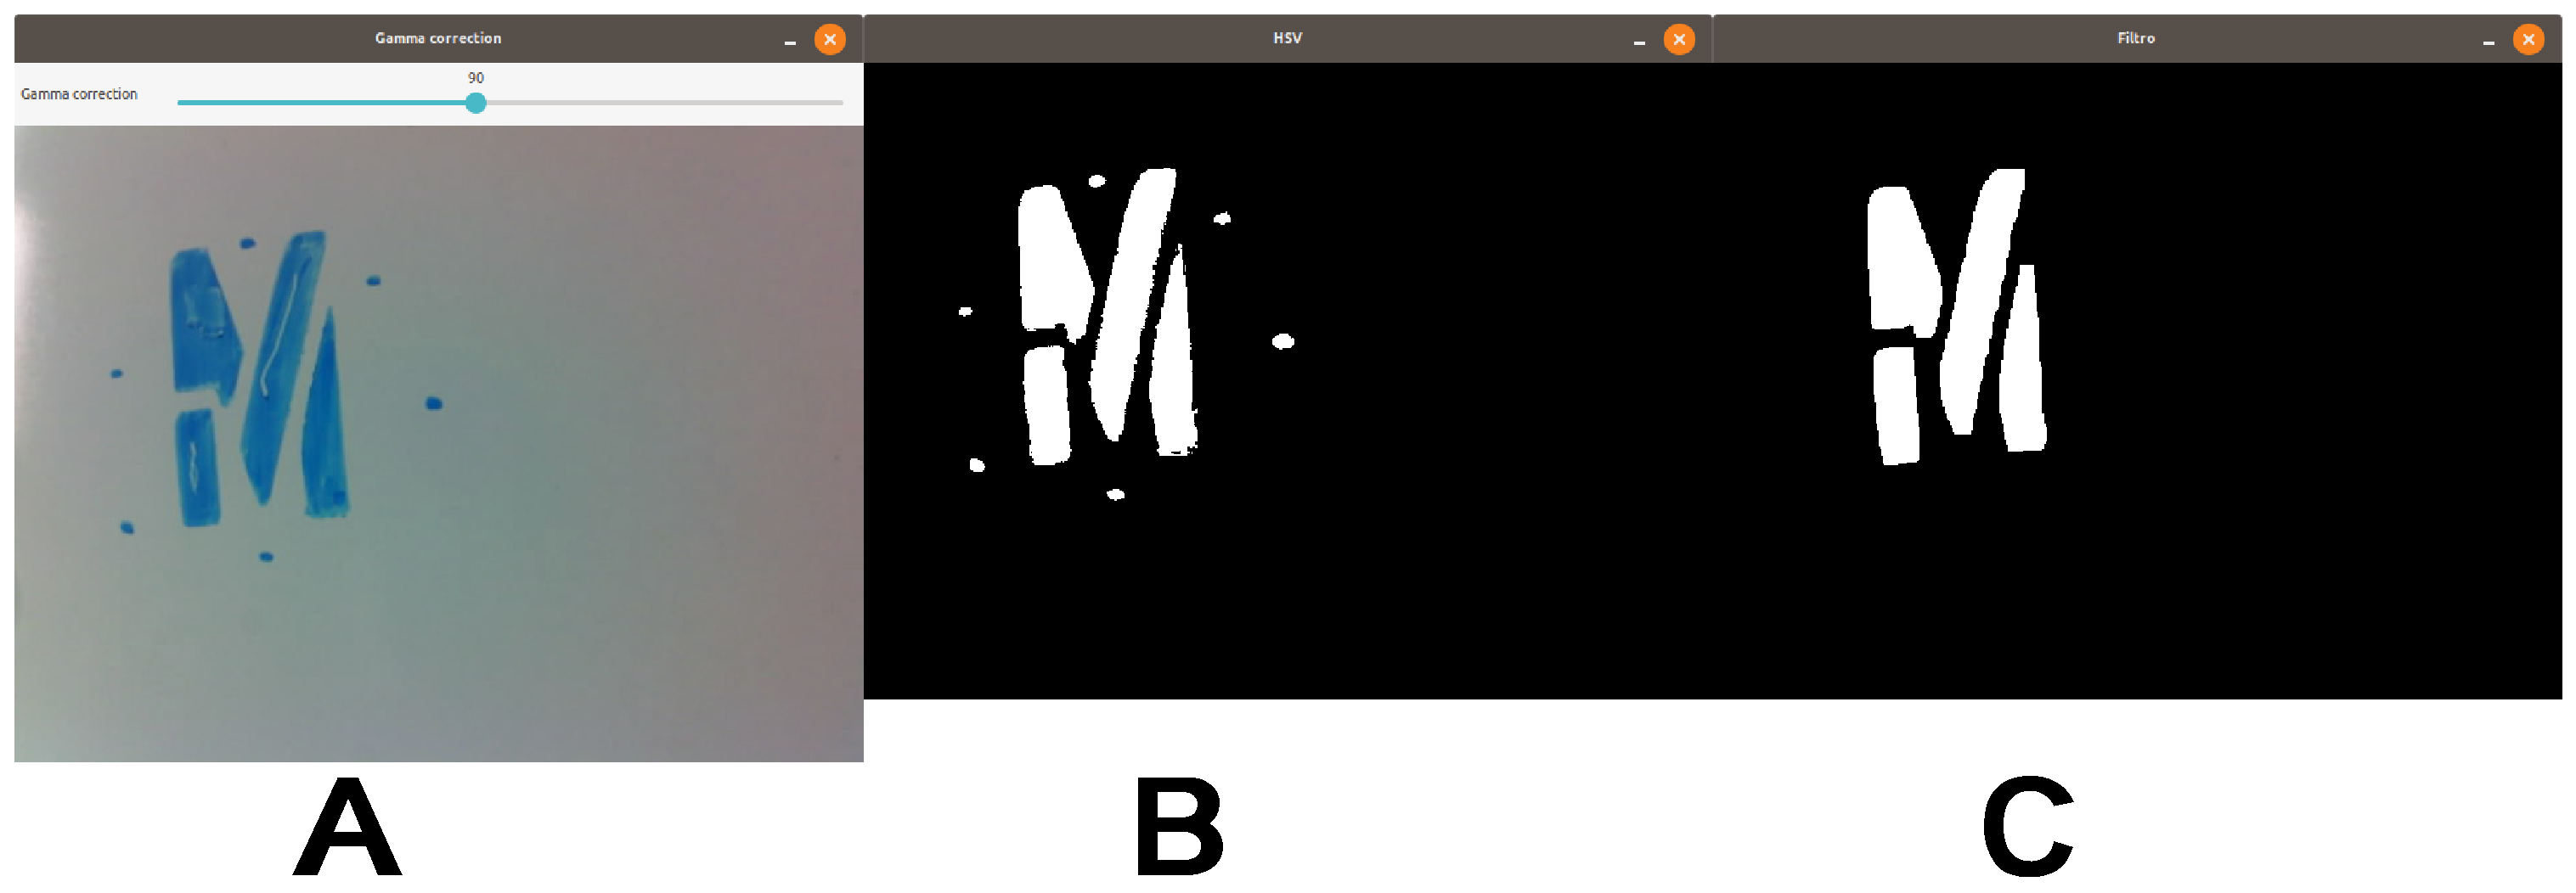
\includegraphics[width=0.6\textwidth]{Contenido/Cuerpo/Capitulo4/Fig15.eps}
	\captionof{figure}{A) Imagen original,B) Espacio de color HSV C)Aplicación de flitros}\label{Fig9}
\end{center}
Con un size de 5 para el kernel del filtro opening se obtuvo un resultado que considero aceptable porque
limpió el ruido externo, es decir, desapareció los puntos que no están asociados con nuestro objeto deseado.

% ---------------------------------------------------------------------------------------------------------
% *********************************************************************************************************
% *********************************************************************************************************
% ---------------------------------------------------------------------------------------------------------

\section{Centroide}
Para obtener el centroide de un objeto en una imagen binaria tenemos que hacer uso del
teorema de green, visto en el capítulo 1, y de las librerías opencv.\\
Para obtener los momentos de la imagen la siguiente función es útil
\begin{example}[label={ex:serie}]{Moments}
	\textcolor{RoyalBlue}{moments(}\textcolor{Bittersweet}{\_Image}\textcolor{RoyalBlue}{)}
\end{example}
Dicha función nos arroja los momentos de la imagen, siendo el m00 el área. La primera
prueba se hizo con cubo rubrik de 3x3, siendo el azul el color target y de dimensión
1.6cm por cada cuadrito de color. Las pruebas se hicieron de noche ambientado con luz
emitida por una seria de leds blancos.
\begin{center}
	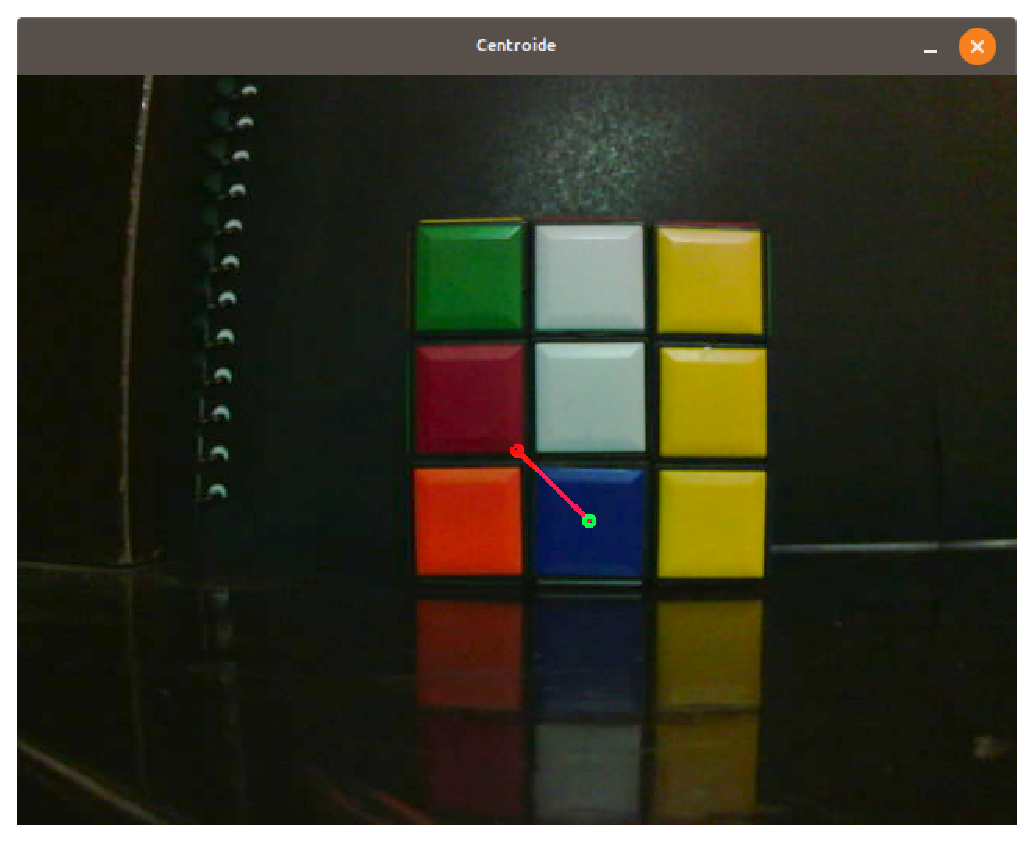
\includegraphics[width=0.6\textwidth]{Contenido/Cuerpo/Capitulo4/Fig18.eps}
	\captionof{figure}{Obtención del centroide del color azul}\label{Fig9}
\end{center}
En la figura anterior podemos observar un punto rojo situado en el origen del sistema
de coordenadas de la imagen, dado en el pixel [320,480]. Debido al ambiente se tuvo
que ajustar gamma a un valor de 60, esto con el objetivo de aclarar los colores
ya que el azul parecía más un negro.\\
El punto verde es el centroide de la figura que está localizado en [366,284], que
a simple vista parece estar en lo correcto, sin embargo hay que comprobarlo. Por lo
que da pie a la siguiente prueba.